% !TEX program = arara
% arara: pdflatex
% arara: biber
% arara: pdflatex
% arara: pdflatex
% arara: clean: { files: [ Paper.out ] }
% arara: clean: { files: [ Paper.aux, Paper.bbl ] }
% arara: clean: { files: [ Paper.bcf, Paper.blg ] }
% arara: clean: { files: [ Paper.log, Paper.run.xml ] }
% arara: clean: { files: [ Paper.toc, Paper-blx.bib ] }
% 

\documentclass{Paper}
\usepackage{todonotes}
\usepackage{xcolor}
\usepackage{pgf-pie}
\usepackage{pgfplots}
\usepackage{float}
\usepackage{textcomp}
\usepackage{subfigure}
\usepackage{filecontents}
\usepackage{pgfplots, pgfplotstable}
\usepgfplotslibrary{statistics}
% define custom colours
\definecolor{greenOfApproval}{HTML}{009933}
\definecolor{redOfDisapproval}{HTML}{cc0000}
\definecolor{yellowOfBrevity}{HTML}{ffcc66}
\definecolor{purpleOfLengthiness}{HTML}{6600cc}

\begin{document}

\maketitle

% % % % %

\tableofcontents
\clearpage
	
\section{Abstract}
	\todo{Autor: Berna}

Jeder Mensch nimmt die Zeit subjektiv unterschiedlich wahr. Dies merkt man doch insbesondere daran, dass die Zeit manchmal wie im Flug vergeht. Andererseits, hat man Momente, da kommen einem fünf Minuten wie eine Ewigkeit vor. Lässt sich dieses, ohnehin subjektiv unterschiedliche Zeitempfinden in der virtuellen Welt durch bestimmte Zeitgeber manipulieren? Kann unser Zeitempfinden also bewusst beeinflusst werden?  Dieser Frage ist eine Gruppe von Studierenden des Studienganges Digitale Medien der Universität Bremen nachgegangen und hat sie anhand eines Experiments beantwortet. Hierzu wurde eine Virtual Reality Welt erstellt, in der 48 Versuchspersonen eine Virtual Reality Brille (Oculus Rift) aufsetzten und sich bewegen mussten. Einige Versuchspersonen wurden durch randomisieren der Welt in verschiedene Bereiche teleportiert. Die Welt wurde in der Unreal Engine erstellt und beinhaltet 3D Objekte, die zuvor in dem Programm Blender erstellt wurden.  Die aufschlussreichen Ergebnisse wurden anhand von Tests, die vor und nach dem Experiment durchgeführt wurden, festgehalten. Bei den Tests ging es darum, das Zeitempfinden des Versuchspersonen genauer zu untersuchen. Dazu sollten die Probanden jeweils 3 Zeitintervalle abschätzen: 30 Sekunden, 40 Sekunden mit Unterhaltung sowie 40 Sekunden ohne Unterhaltung. Des Weiteren wurde ein IQ Test durchgeführt sowie die Temperatur jeder Versuchsperson gemessen, um die Ergebnisse optimal auswerten zu können. Die Ergebnisse wurden anschaulich anhand von Graphen dargestellt sowie interpretiert.



\section{Einleitung}
\todo{Autor: Kim}
\subsection{Einstieg}

In den letzten Jahrhunderten unverkennbar zu beobachten ist ein enormer Wandel unserer Gesellschaft auf technischer sowie sozialer Ebene.
Eine Zunahme der Relevanz des Begriffes „Zeit“ ist durch die öffentlichen Diskussionen über Stress, Burn-Out oder dergleichen zu beobachten.
Immer mehr Menschen der arbeitenden Gesellschaft leiden unter diesen Phänomenen, die auf „zu wenig Zeit“ zurückzuführen sind. Das zunehmende Interesse der Themen Effizienz, Schnelligkeit und Leistung ist außerdem unübersehbar. Die Gesellschaft versucht immer schneller und immer mehr Arbeiten in einer kürzeren Zeit zu erledigen. Dies ist ganz offensichtlich auch auf die Industrialisierung und auf das zunehmende Tempo der Gesellschaft zurückzuführen. Wo früher noch Tage auf die Antwort eines Briefes gewartet wurde, ist es heute möglich innerhalb weniger Minuten ganze Arbeitsschritte oder Anweisungen via Email zu kommunizieren und anschließend die erwarteten Leistungen zu erbringen.
Des Weiteren lässt sich beobachten, dass die Arbeits-und Schlafzeiten der arbeitenden Bevölkerung massiv gesenkt wurden.
\\
Daraus ergibt sich nun die Bildung der Freizeit und somit die Notwendigkeit des Zeitmanagements. Jeder versucht seine Tage optimal zu nutzen und einzuteilen, um noch genug Zeit für die Freizeit und Familie zu haben. Des Weiteren schaffen auch die neuen Entwicklungen der Industrialisierung wie Handy, Mikrowelle, Computer und weitere technische Erfindungen mehr Zeit für jeden Einzelnen. Dennoch sind Versuche, die Zeit durch immer effizientere und „zeitsparendere“ Abläufe zu bändigen nur Scheinerfolge: Die Zeit vergeht trotzdem gleichförmig und schleichend unaufhaltsam und unwiderruflich weiter. Es besteht also ein hohes Interesse in der Erforschung dieses Gebietes, um die Zeit, die jedem Einzelnen zur Verfügung steht, optimal zu nutzen.

Dennoch steht uns immer noch derselbe biologische Apparat zur Verfügung. Zeit vergeht immer gleich schnell. Doch die Frage ist: Ist das wirklich so ? Vergeht die Zeit immer gleich schnell oder gibt es bestimmte Indikatoren, die uns die Zeit als schneller oder langsamer vergehend vorkommen lassen ? Kann man das Zeitempfinden also beeinflussen?

\subsection{Fragestellung }
Dies führt uns zu unserer Forschungsfrage: \textbf{Kann man das Zeitempfinden in der Virtuellen Welt durch bestimmte Zeitgeber manipulieren?}\\
Als Zeitgeber definieren wir Alltagsumgebungen, Phänomene der allgemeinen Lebenswelt und physische Kräfte, die uns unter Ausschluss der Uhrzeit, die Zeit vorgeben.
Wir konzentrierten uns auf die Zeitgeber einer verschnellerten und verlangsamten Gravitation, so wie einem verschnellerten und verlangsamten auditiven Zeitgeber in Form eines Tickens an der Ampel. Wir erschufen eine visuell an Alltagssituationen angelehnte virtuelle Welt, die Szenarien aufzeigt, die jeder Mensch tagtäglich erlebt.

Nach Ablauf der Strecke wurde die Versuchsperson mit Hilfe eines Fragebogens zu seinen Eindrücken in der virtuellen Welt befragt und durch die „Four Alternative Forced Choice“ - Methode „gezwungen“, die einzelnen erlebten Szenarien nach ihrer Dauer zu sortieren. So erhofften wir uns herauszufinden, ob eine der erlebten Manipulationen die Zeitwahrnehmung der Versuchsperson rafft oder streckt. Mit Hilfe von Statistik (siehe Kapitel 2 „Methodik“) ließ sich nun herausfinden, ob eines der Manipulations-Szenarien überproportional auffällig von allen Versuchspersonen als kürzer bzw. länger eingestuft wurde als andere Szenarien und wir somit eine Manipulation der Zeit erzeugen konnten. 
\par
Ein weiterer Fokus unserer Arbeit bezieht sich auf die Zeiteinschätzung vor und nach dem Befinden in der Virtuellen Welt:
\textbf{Unterscheidet sich die Zeiteinschätzung der einzelnen Versuchspersonen vor und nach dem Befinden in der Virtuellen Welt ?} Verändert also das Erlebnis, sich in einer nicht reellen Welt zu befinden das Zeitempfinden ?
Unter Betrachtung des Spaßfaktors, der auch einen erheblichen Einfluss auf die Zeitwahrnehmung nimmt, wurden alle Versuchspersonen zusätzlich gebeten, die Dauer bestimmter Zeitintervalle jeweils vor und nach dem Befinden in der Virtuellen Welt einzuschätzen. Wenn die Versuchspersonen der Meinung waren, das die Zeitintervalle vorbei waren ( 40 Sekunden, 40 Sekunden mit Unterhaltung, 30 Sekunden ) sollten sie es durch ein Zeichen kenntlich machen. Zusätzlich wurde sich bei einem der Einschätzungsintervalle mit den Versuchspersonen unterhalten, um ebenfalls herauszufinden, ob Ablenkung einen Einfluss auf die Zeitwahrnehmung nehmen konnte.


\subsection{Hypothesen}

Bezüglich unserer zwei Forschungsschwerpunkte haben wir folgende Hypothesen erstellt:
\begin{enumerate}
\item „Visuelle und auditive Zeitgeber verändern das Zeitempfinden der Versuchsperson in der virtuellen Welt“
par\
Wir vermuten, dass die Manipulation der Zeitgeber in einer virtuellen Welt die Zeitwahrnehmung verändert und die Zeit somit schneller oder langsamer vergeht.

\item „Der Spaßfaktor in der Virtuellen Welt hat einen Einfluss auf die Zeitwahrnehmung der Versuchsperson.“
par\
Der Spaßanteil, den man während einer Aktion erlebt, hat großen Einfluss auf die Zeitwahrnehmung und kann die vergangene Zeit raffen oder im Falle von geringem Spaßfaktor strecken.


\item „Das Befinden in der Virtuellen Welt verändert das Zeitempfinden nach Rückkehr in die reale Welt“
par\
Wir vermuten, dass das Befinden in der Virtuellen Welt die allgemeine Wahrnehmung und somit auch das Zeitempfinden kurzzeitig beeinflussen und verändern kann.
\end{enumerate}




\subsection{Ziel der Arbeit}
Das Ziel der Arbeit ist es, die zuvor genannten Hypothesen zu belegen bzw. zu widerlegen und somit, unter anderem, herauszufinden, ob man die Zeitwahrnehmung einzelner Menschen mithilfe der Manipulation von Zeitgebern verändern kann. Mithilfe der virtuellen Welt war dieses Experiment für uns umsetzbar und die Frage bleibt offen, ob man eine solche Zeitmanipulation auch in der realen Welt durchführen könnte. Das Belegen der Hypothesen wäre ein wichtiger Wegweiser für weitere Forschungen in diese Richtung.\\
Das Ziel dieser Arbeit ist es nicht, dieses Forschungsfeld abzuschließen, sondern versucht nur, es anzustoßen und Freiraum für weitere Experimente zu schaffen.

\subsection{Datenbasis/Forschungsstand}
Diese Arbeit bezieht sich auf und orientiert sich an verschiedenen Studien zur Zeitwahrnehmung und Zeitmanipulation in der Virtuellen Welt. \\
Eine davon untersucht, ob die Veränderung der Sonnenzirkulation in der Virtuellen Welt einen Einfluss auf die Zeitwahrnehmung nehmen kann. Auch diese Forschungsgruppe benutzte verschiedene Zeitgeber, um eine Manipulation des Zeitempfindens hervorzurufen. Diese Zeitgeber waren: Die Sonne ohne Bewegung, die Sonne im normalen 24 Stunden-Zyklus und eine Sonne, die sich doppelt so schnell bewegte, wie der normale 24 Stunden Zyklus der Sonne. Die Versuchspersonen wurden in drei Gruppen aufgeteilt, die jeweils andere Aufgaben zu erledigen hatten. Eine Gruppe sollte nichts machen und nur auf einem Stuhl sitzen. Eine weitere Gruppe hatte eine sprachliche, kognitive Aufgabe und eine weitere Gruppe sollte eine „räumliche“ Aufgabe erfüllen.
Diese Forschungsgruppe kam zu folgendem Ergebnis: Wenn die Versuchspersonen nichts zu tun hatten und nur auf einem Stuhl saßen, überschätzten sie die Zeit und die Sonnenbewegungen hatten einen großen Einfluss auf ihre Zeitwahrnehmung. Wenn sie aber währenddessen mit einer Aufgabe beschäftigt waren, unterschätzten sie die Zeit, die in der VR vergangen war und es gab keine Unterschiede in der Zeitwahrnehmung zwischen den verschiedenen Sonnenzyklen.
\par
Eine weitere Studie, die uns wichtige, zu beachtende Faktoren zur Zeitmessung vorgab, ist Pascal Wallisch' wissenschaftlicher Bericht „Zeiterleben in der Tempogesellschaft“.  \\
Wallisch beschreibt, \glqq dass das menschliche Zeitempfinden, insbesondere die Empfindung von Dauer von allen möglichen Faktoren abhängig ist\grqq .( S. 27 ) \\
Für unser Experiment ist es von bedeutender Wichtigkeit, dass keiner der Versuchspersonen in seiner Zeitempfindung durch Faktoren beeinflusst wird, um sicherzustellen, dass korrekte Ergebnisse resultieren.
Für uns galt es also mit Hilfe eines Fragebogens, die von Wallisch’s beschriebenen Einflüsse und Faktoren vor dem Experiment für jede Versuchsperson abzufragen, auszuschließen bzw. in unserer Ergebnisse einzubeziehen und separat zu betrachten, falls die einzelnen Messwerte oder Angaben außerhalb des Rahmens liegen und zu veränderten Zeitschätzungen führen könnten. Nur so können wir abweichende Ergebnisse begründen und auf veränderte Einflussfaktoren beziehen.\\
Zu diesen Einflüssen gehören unter anderem die Intelligenz, das Alter, Geschlecht, Drogen-und Medikamenteneinflüsse, Müdigkeit ( nur bedingt, da Müdigkeit nur die Ereignis-Fusions Schwelle senkt und nicht direkt die Zeitwahrnehmung verändert ( siehe S. 28 bzw. Kapitel 3.3 )), Körpertemperatur, Gehirnschäden und psychische Erkrankungen.
\\Außerdem betrachteten wir den Artikel „Warum Jahre rasen und Sekunden schleichen“ , dieser veranschaulicht, dass auch das Spaßempfinden einen Einfluss auf die Zeitwahrnehmung nimmt. So integrierten wir den Spaßfaktor als weiteres zu beachtendes Kriterium in unseren Fragebogen A.


\subsection{Aufbau der Arbeit}
Diese vorliegende Forschungsarbeit stellt einen Versuch dar, sich der Möglichkeit der Zeitmanipulation zu nähern, indem zunächst - nach einem kleinen historischen Überblick über die Entwicklung von Zeit - das Ziel der Arbeit, sowie die Vorgehensweise des Experiments erläutert wird. Des Weiteren wird auf den Forschungsstand in diesem Gebiet eingegangen und Foschungshypothesen werden erstellt. Aus diesen wird eine sinnvolle Methodik abgeleitet, vorgeschlagen und durchgeführt, insofern dies mit den gegebenen Mitteln machbar erschien. Deren Resultate werden in einem abschließenden Teil im Sinne der Fragestellung und der Hypothesen aufgeführt, interpretiert, diskutiert und zukunftsorientiert betrachtet. Zum Schluss rundet ein Fazit die Forschungsarbeit ab.



 
	
\section{Methode}
	\todo{Autor: Nizan \& Alina}
	\subsection{Methodik}
	\par
		Die wissenschaftliche Methode des Experiments war die Grundlage unseres Projekts, anhand der wir unsere Leitfrage und Hypothesen auf ihren Wahrheitsgehalt untersuchten um Zusammenhänge darzustellen.
		Es galt bestimmte Untersuchungs-Anordnungen zu berücksichtigen, um so die Erhebung von Daten zur Zeitwahrnehmung zu sichern, aufbauend auf bereits bekannten Erfahrungswerten.
		
	\par
		Vorteile dieser Methode war eine kontrollierte Laborsituation, in denen alle Bedingungen und
		Abläufe unter den gleichen Voraussetzungen stattgefunden haben. Dadurch wurden äußerliche
		Einflussfaktoren, die das Verhalten hätten beeinflussen können verhindert. Alle für die
		Fragestellung relevanten Faktoren konnten anhand der Laborbedingungen kontrolliert werden.
		Dadurch wurde eine Wiederholbarkeit gewährleistet, die ermöglicht, das Experiment bei Bedarf
		zu wiederholen, zu Überprüfungs- und Forschungszwecken oder bei Ausfällen.
		\par	
			Ein Nachteil dieser Methode ist die Frage der Ethik. Die Untersuchung menschlichen Verhaltens
		mit dem Ziel an Forschungsergebnissen zu gelangen, ist etwas problematisch. Besonders,
		wenn die Manipulation im Rahmen eines Experiments die Persönlichkeit eines Menschen
		langfristig prägen oder beeinflussen könnte. Deshalb wurde sich bei der Themenwahl strickt an die
		ethischen Richtlinien gehalten, um den Fortschritt und gleichzeitig die Sicherheit der zu
		testenden Personen zu gewährleisten. Die Versuchspersonen wurden weitestgehend über
		Zweck und Ablauf des Verfahrens sowohl als über die vorhersehbaren Unannehmlichkeiten sowie
		Risiken informiert. Des Weiteren wurde der Proband über den zu erwartenden Nutzen
		aufgeklärt und hatte die Möglichkeit das Experiment jeder Zeit auf Wunsch abzubrechen.
		\par	
Beim wissenschaftlichen Arbeiten gilt es einige grundsätzlichen Kriterien zur Sicherung der Qualität einzuhalten. Diese sind Ehrlichkeit, Objektivität, Überprüfbarkeit, Logik, Originalität, Validität 
und Verantwortung auf deren Einhaltung wir großen Wert gelegt haben.\\
Das Ziel dieser Arbeit war es nicht, dieses Forschungsfeld abzuschließen, sondern lediglich diesem einen Anstoß zu geben, um einen Freiraum für weitere Experimente zu schaffen. Diese Forschungsarbeit versucht ein Themenfeld zu erkunden, zudem man nur wenige Veröffentlichungen findet, um somit vielleicht einen kleinen Meilenstein in der Erforschung der Zeitwahrnehmung zu setzten.		

	
	\subsection{Versuchspersonen}
		Fünfzig Versuchspersonen im Alter zwischen 18 und 80 Jahren (Mittelwert lag bei 31 Jahren),
		davon 35 Männer und 13 Frauen, unterschiedlichen akademischen Grades und Berufs, nahmen
		freiwillig am Experiment teil. Achtundvierzig teilnehmende Personen waren für die
		Durchführung nötig, da die vier Szenarien in vierundzwanzig verschiedenen Reihenfolgen
		dargestellt werden konnten. Diese sollten jeweils von zwei Personen durchgeführt werden. Die
		Verteilung verlief anhand des Zufallsprinzip. Es wurde keine Entschädigung angeboten. Alle
		Probanden hatten nach eigenen Angaben normale oder mit Brille bzw. Kontaktlinsen auf
		normal korrigierte Sehkraft und normales Farbsehen. Personen mit
		psychischen Erkrankungen, Gehirnschäden oder schlechten Deutschkenntnissen wurden in den Unterlagen vermerkt. Die Versuchspersonen waren bezüglich der experimentellen Hypothese unwissend
		und unterschrieben vor der Teilnahme eine schriftliche Einverständniserklärung mit allen
		Risiken und datenschutzrechtlichen Informationen.
		Von der Endauswertung ausgeschlossen wurden zwei Personen die Aufgrund von Übelkeit und
		Schwindel das Experiment vorzeitig beenden mussten.
		\par
		
		\footnote{$()$}
		
	\subsection{Apparaturen}
		Zwei Räume wurden für die Durchführungen des Experiments genutzt. Im ersten Raum, in dem der erste und letzte Teil des Experiments stattfand, wurden die Befragungen und Zeiteinschätzungs-Tests gemacht. 
	Die Versuchsperson saß den Testern an einem Tisch gegenüber. Die benötigten Materialien (Probandenmappe, Stoppuhr, Infrarot-Thermometer, Schutzkappen) lagen bei den Testenden. Zu der Probandenmappe gehören folgende Dokumente:\\		
	 (1) Einverständniserklärung, (2) \glqq Fragebogen B\grqq, (3) \glqq Fragebogen A\grqq, (4)
		Mehrfach-Wortschatz-Intelligenztest und (5) \glqq Fragebogen C\grqq.
		Diese wurden, in Klemmbrettern geordnet, für die Durchläufe mit den Versuchspersonen
		vorbereitet. \\
		Im zweiten Raum fanden die VR-Experimente statt. Dort stand ein Drehstuhl, um sich flexibel in der
		Welt bewegen und drehen zu können; ein Tisch mit einem Computer (Windows 10) und zwei Monitore auf denen man
		die virtuelle Welt sehen und mit der Unity Software bearbeiten konnte; Kopfhörer um äußere
		Geräusche zu minimieren und die Audio und Hintergrundgeräusche hören zu können; die Oculus DK2 VR-Brille
		zur Orientierung in der VR und ein Xbox-Controller für die Steuerung in der Welt.

	\subsection{Prozedur}
Das Experiment fand in einer Laborsituation unter kontrollierten Bedingungen statt. Die
Ergebnisse des Experiments sind unabhängig vom Versuchsleiter zustande gekommen. Dank
eines strengen Ablaufplans und Briefings waren alle Projektmitglieder im Stande jeden Schritt im Experiment betreuen zu können. Die interne Validität der Messungen waren daher sehr genau und
objektiv. Der Zeitraum der Experimentdurchführung lag bei sechs Tagen, in denen jeweils im
Durchschnitt 8.3 Versuchspersonen an der Untersuchung teilnahmen. Jeder Durchlauf hat je
nach Proband zwischen 25 Minuten bis 40 Minuten gedauert.
\par
Der Ablauf des Experiments bestand aus drei Teilen. Der theoretische Teil vor der VR, der
praktische Teil in der VR und der theoretische Teil nach der VR. Die Messmethode war
aussagekräftig, da alle Durchläufe sowie die dazugehörigen Erklärungen bei allen Probanden
exakt gleich stattgefunden haben.

\subsubsection{Theoretische Teil vor der VR}
Jeder Durchgang begann mit einer Einweisung durch die Räumlichkeiten. Der erste Teil des
Experiments fand in einem separaten Theorieraum ,,Raum 1'' statt. Experimentator und
Proband saßen sich gegenüber an einem Tisch. Der Proband unterschrieb eine
Einverständniserklärung. Ein Zeiteinschätzungs-Test wurde durchgeführt, in dem der
Proband 40 Sekunden ohne Hilfsmittel einschätzen sollte, ohne sich zu unterhalten.
Das Ergebnis wurde von einem der anwesenden Experimentatoren anhand einer Stoppuhr
gemessen und auf dem „Fragebogen B“ erfasst. \\
Der Proband bekam den „Fragebogen A“ ausgehändigt. Es sollte angegeben werden (1) ob die zu testende Person unter
Drogeneinflüaawn steht, (2) wie der akute Müdigkeitswert ist, (3) ob und an welchen
Gehirnschäden oder psychischen Erkrankungen die Person leidet und (4) welche die
Muttersprache der Versuchsperson ist. 
\par
Ein Intelligenztest (MWT-B) wurde durchgeführt. Bei
dem angewandten Intelligenztest handelte es sich um den psychologisch anerkannten
„Mehrfach-Wortschatz-Test (MWT-B)“, entwickelt von Siegfried Lehrl \cite{MWT-B}. Der Test wurde aus
der sogenannten „Testothek“ der Universität Bremen ausgeliehen, nach Empfehlungen des
Psychologie Studenten Till Rachwitz, der sich auf die Durchführung von Intelligenztests
spezialisiert hat. Dieser begründete die Wahl dieses Tests damit, dass er simpel und kurz
durchzuführen ist. Er bietet einen groben Überblick über die allgemeine Intelligenz
einzelner Personen. Zwar geht er nicht auf einzelne Schwerpunkte wie Logik, Mathematik
oder Psychologie ein, misst aber die allgemeine Intelligenz und ist zudem objektiv, robust
und benötigt einen geringen Materialaufwand. Im MWT-B gilt es aus 37 Wortreihen,
bestehend aus jeweils vier fiktiven und einem existierendem deutschen Wort, das korrekte
Wort zu finden und durchzustreichen. Es gab
keine zeitliche Begrenzung und keine Hilfestellung.
\par
Ein erneuter Zeiteinschätzungs-Test wurde durchgeführt, in dem die Versuchsperson 40 Sekunden abschätzen und sich gleichzeitig mit den Experimentatoren unterhalten sollte. \\
Anschließend wurde die Körpertemperatur des Probanden mithilfe des Infrarot-Thermometers am Ohr gemessen und anschließend ein 30 Sekunden
Zeiteinschätzungs-Test ohne Gespräch durchgeführt. Alle Ergebnisse der Zeiteinschätzungen und die
Körpertemperatur wurden von dem Experimentator auf dem vorgedruckten ,,Fragebogen B''
notiert. Der Proband hatte keine Einsicht auf die Ergebnisse.

\subsubsection{Praktische Teil in der VR}
Der zweite Teil findet in einem isolierten ,,Raum 2'' statt. Der Proband
bekam die Anweisung, sich auf ein Drehstuhl zu setzen. Weitere Anweisungen für die
Durchführung vom Experiment waren: (1) Die Fortbewegung findet mittels eines Xbox-
Controllers statt, (2) Man kann sich frei durch die Welt bewegen, (3) Anhand der VR-Brille
kann man sich umsehen, (4) Man sollte sich an die allgemeinen Verkehrsregeln halten, (5)
Die Umgebung sollte einprägt werden für spätere Befragungen.
\par
Die Oculus DK2 VR-Brille und Kopfhörer wurden der Versuchsperson aufgesetzt und der Controller in die Hand gelegt. Zu Beginn des Experiments wurde die Zeit gestoppt, die der Proband für die
gesamte Strecke der vier Szenarien benötigt. Erfasst wurde die Zeit vom Zeitpunkt des Loslaufens bis zur Ankunft am Schild ,,Road Closed''. \\
Die insgesamt vier Szenarien bildeten die
virtuelle Welt und bestanden aus vier Ampelphasen. Diese waren visuell und auditiv einer
realen Welt nachgebaut mit Wegen, Straßenverkehr, Autolärm, Menschen, Häusern und
Bäumen. 

\begin{figure}[H]
\centering
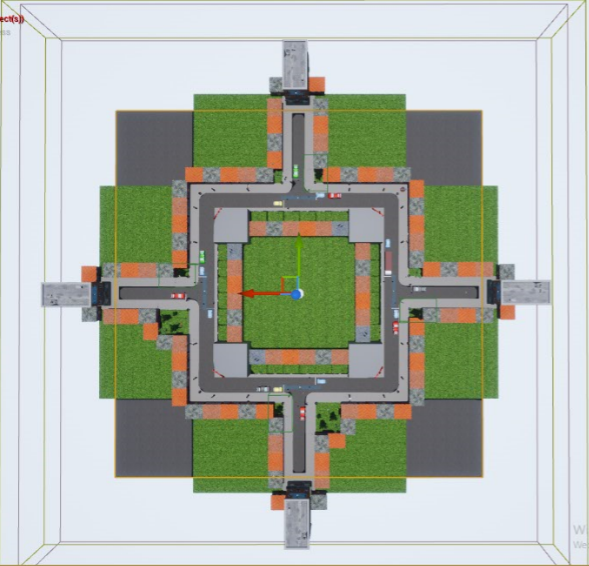
\includegraphics[scale=0.6]{bilder/map.png}
\caption{Ansicht der virtuellen Welt von oben, wo an jeder Ampel eins der Szenarien stattfindet.}
%\label{}
\end{figure}

An jeder Ampelphase gab es einen manipulierten Faktor, der die
Zeitwahrnehmung beeinflussen soll. Immer zwei der Szenarien gleichen sich optisch, haben aber gegenteilige Zeitgeber. (a) Ampelphase an einem LKW - schnelles Ticken, (b) Ampel mit Vogel und
Menschen - langsames Ticken, (c) Ampel neben einem schaukelndem Kind mit rosa Shirt -
schnelles Schaukeln, (d) Ampel mit Heißluftballon-Plakat bei einem schaukelndem Kind mit
grünem Shirt - langsames Schaukeln.

\begin{figure}[H]
    \subfigure[Ampelphase an einem LKW]{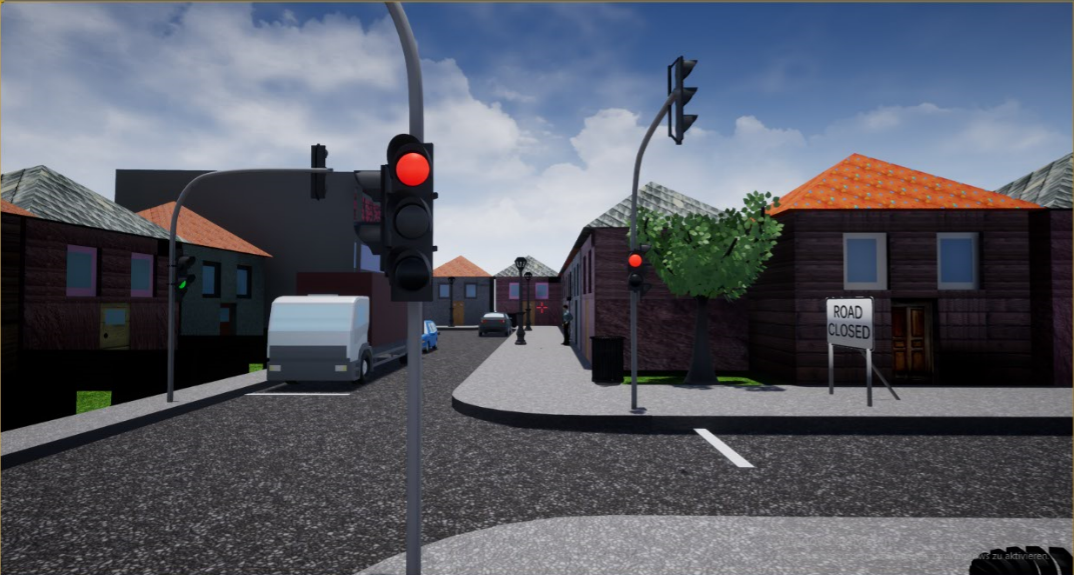
\includegraphics[width=0.5\textwidth]{bilder/a.png}}
    \subfigure[Ampelphase mit Vogel und
Menschen]{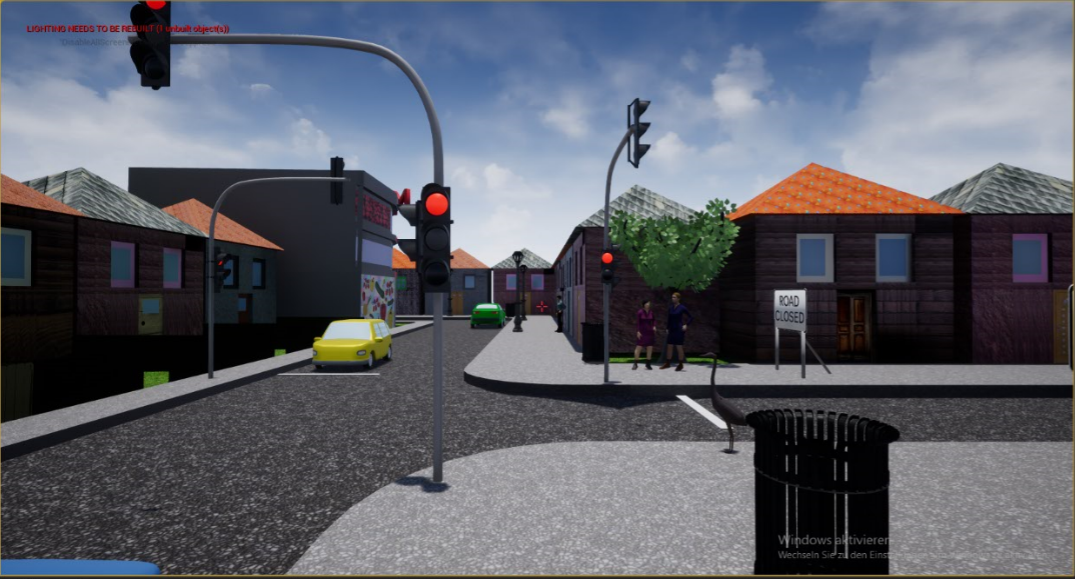
\includegraphics[width=0.5\textwidth]{bilder/b.png}}
%\caption{Titel unterm gesamten Bild}
\end{figure}

\begin{figure}[H]
    \subfigure[Ampel neben einem schaukelndem Kind mit rosa Shirt]{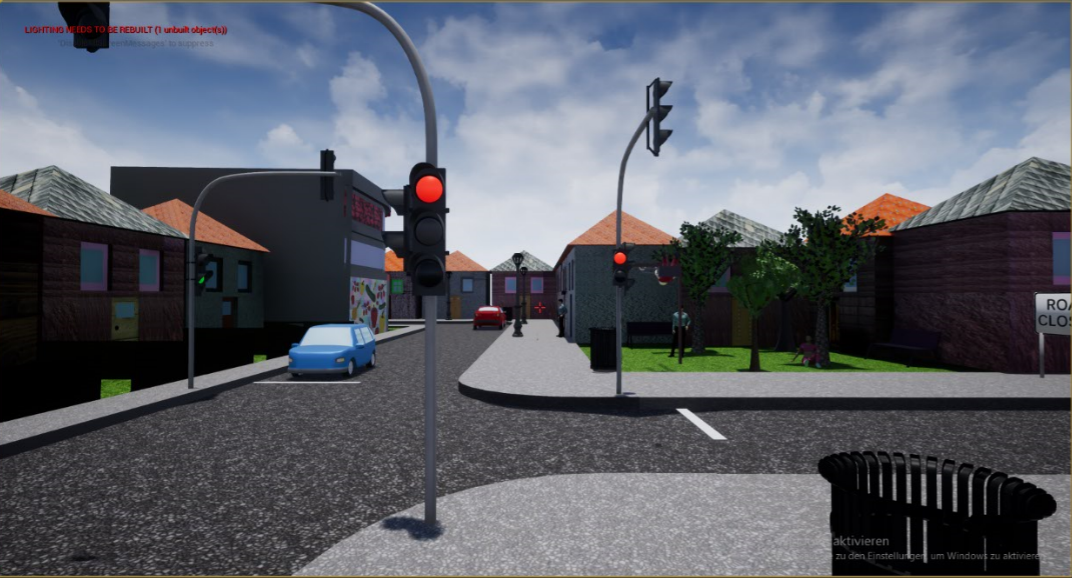
\includegraphics[width=0.5\textwidth]{bilder/c.png}}
    \subfigure[Ampel neben einem schaukelndem Kind mit
grünem Shirt]{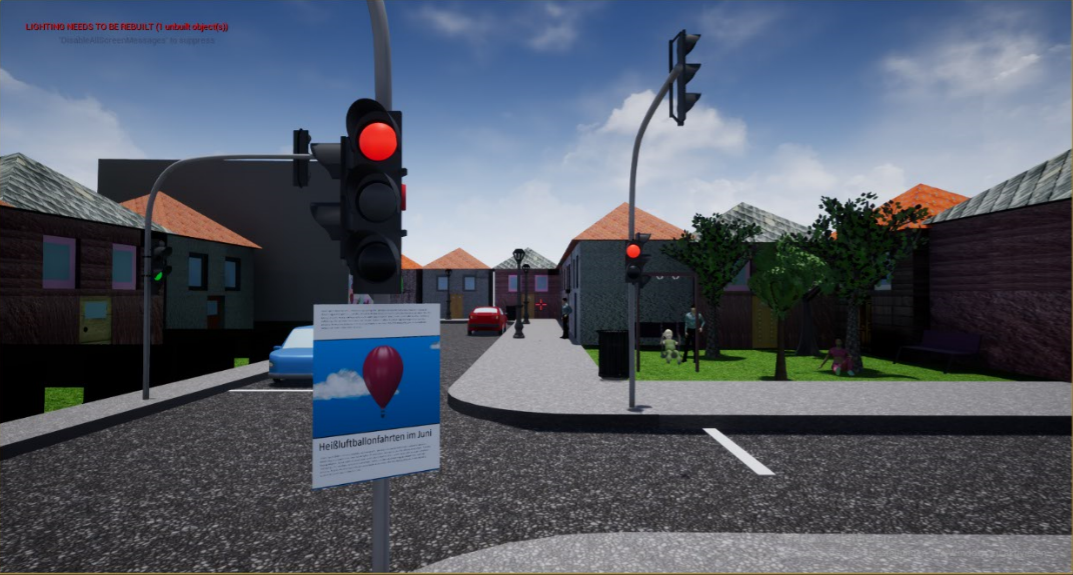
\includegraphics[width=0.5\textwidth]{bilder/d.png}}
%\caption{Titel unterm gesamten Bild}
\end{figure}

Die Wartezeit an den Ampeln war vorgegeben und konnte nicht frühzeitig übersprungen werden. Der Proband durchlief die virtuelle Welt einmal und ohne Unterbrechungen. Die Geschwindigkeit in der die Welt durchlaufen wurde, konnte die
Versuchsperson selbst anhand des Controllers regulieren. Die Versuchsleiter konnten das
Geschehen in der VR über die Bildschirme beobachten. Es wurden
keine weiteren Anweisungen noch eine zeitliche Begrenzung vorgegeben. 


\subsubsection{Theoretische Teil nach der VR}
Nach der VR wird der Proband wieder im ersten Raum auf verschiedene Dinge getestet.
40 Sekunden ohne
Unterhaltung wurden abgeschätzt und vom Versuchsleiter erfasst. Der Proband erhielt
„Fragebogen C“ und sollte angeben: (1) die geschätzte Dauer von den einzelnen Szenarien
(2), die besten und schlechtesten empfundenen Szenarien, (3) die empfundene Dauer in
der virtuellen Welt, (4) den eigens empfundenen Spaßfaktor, (5) auffallende
Besonderheiten in der virtuellen Welt und (6) eine Einschätzung, worum es in dem
Experiment ging.
\par
Ein erneuter Zeiteinschätzungs-Test wurde durchgeführt, in dem die
Versuchsperson 40 Sekunden abschätzen und sich gleichzeitig mit einem der Versuchsleiter
unterhalten sollte. Die Ergebnisse wurden erneut vom Versuchsleiter notiert. Zum Schluss fand ein 30
Sekunden Zeiteinschätzungs-Test ohne Gespräch statt. 
Die Versuchsperson durfte ihre Zeiteinschätzungs-Ergebnisse auf Wunsch erfahren, sowie das Ergebnis vom
Intelligenztest. Räume und Klemmbretter für den nächsten Probanden wurden vorbereitet.
\par
	\subsection{Begründung des Aufbaus der Szenarien}

Für unser Experiment war es ein wesentlicher Bestandteil, dass die Probanden keinen Unterschied bemerken, wenn sie durch die Teleporter von einem Szenario zum nächsten teleportiert wurden. Daher musste unsere Versuchswelt so konzipiert werden, dass alles gleich aussieht. Die Teleporter wurden so platziert, dass sich die Triggerbox, durch die die Versuchspersonen gingen, direkt nach dem Szenario, also nach der jeweiligen Ecke befindet und die Testperson nicht um die nachfolgende Ecke schauen kann.\\
Der Grund ist, dass die Probanden so mit Sicherheit alle Szenarien sehen und jede Gruppe der Probanden eine unterschiedliche Reihenfolge an Szenarien erlebt. Die Reihenfolge konnten wir jederzeit manipulieren, um zu verhindern, dass gleiche Reihenfolgen direkt hintereinander gezeigt werden und eine Reihenfolge als Begründung für ein spezifisches Ergebnis ausgeschlossen werden konnte. .\\
Die Zeitwahrnehmung sollte durch visuelle und auditive Zeitgeber manipuliert werden. In zwei der Szenarien (\textbf{c}, \textbf{d}) befand sich ein Kind, das jeweils langsam  (\textbf{d}) oder schnell (\textbf{c}) schaukelte und so die Zeit durch verlangsamte oder beschleunigte Gravitation manipulieren sollte. Die Versuchspersonen hatten so während der Wartezeit an der Fußgängerampel etwas zu sehen und wurden so möglicherweise beeinflusst. Die Wartezeit an jeder Ampel beträgt 18 Sekunden und wurde duch eine Triggerbox ausgelöst, über die die Versuchsperson läuftt. \\
Die auditive Manipulation stellte ein gleichmäßiges Ticken an zwei weiteren Szenarien (\textbf{a}, \textbf{b}) dar. Dies sollte ebenfalls das menschliche Zeitempfinden der Testpersonen manipulieren. Während die Versuchspersonen an der roten Ampel warten und ein schnelles Ticken (\textbf{a}) hören, sehen sie zusätzlich einen großen LKW neben sich stehen, der dazu verhelfen soll, dass sich die Probanden hinterher an das Szenario besser erinnern.
Bei dem langsamen Ticken (\textbf{b}) sehen die Probanden einen Vogel an der Ampel und zwei Menschen auf der anderen Straßenseite. Dies dient ebenfalls zur Erinnerung an das jeweilige Szenario.  \\
Der Unterschied zwischen den auditiven und visuellen Manipulationen ist vor allem jener, dass sich die Probanden bei den visuellen Zeitgebern bewusster darauf einlassen, was sie in der VR sehen, da dies in dem Moment der stärkste Sinneseindruck ist.\\


	\subsection{Begründung der Wartezeiten und Zeitabschätzungen}
		Die Wartezeit pro Szenario beträgt genau 18 Sekunden. So bietet die VR-Welt eine realistische Wartezeit an einer Ampel (tatsächliche Ampelzeiten wurden vorher gemessen). \\
18 Sekunden ist eine angemessene Dauer für unser Experiment, da es die Probanden einerseits ungeduldig machtm wann und wie es nun weiter geht und andererseits die Möglichkeit bietet, sich drauf einzustellen jetzt erst einmal warten zu müssen und somit den Effekt erzielt, dass sich die Testpersonen in der Versuchswelt umsehen und die oben genannten Szenarien (\textbf{a}, \textbf{b}, \textbf{c}, \textbf{d}) entdecken, die die Empfindung der Wartezeit beeinflussen sollen.

\section{Ergebnisse}
Wir hatten 48 Probanden, davon waren 13 Frauen und 35 Männer mit einer Altersspanne von siebzehn bis achtzig Jahren. Außer vier Testpersonen waren alle deutsche Muttersprachler und eine Mehrheit von 32 Personen hat unserem IQ-Test zufolge eine durchschnittliche Intelligenz.

\subsection{Scatterplots}
Folgende Streudiagramme zeigen die ersten Daten, die von den Probanden erhoben wurden. Erste Zeiteinschätzungen werden in Relation zu Alter, Intelligenz, Körpertemperatur und Müdigkeit der Probanden gestellt.
Die Streudiagramme sind gruppiert nach den Einschätzungen, die Probanden entweder \textit{ohne} oder \textit{mit} Gespräch absolviert haben: die ersten acht Diagramm zeigen je die 40 bzw. 30 Sekunden-Einschätzungen in Relation zu oben genannten Parametern. Die darauffolgenden acht Diagramme zeigen 40 Sekunden Zeiteinschätzung während der Proband sich unterhält.\\
Zu unterscheiden sind hier die Helligkeiten der Kreise, welche das Geschlecht des Probanden indizieren. Rote Kreise stellen hier die weiblichen Probanden dar und blaue Kreise die männlichen.
%%%%%%%%%%%%%%%%%%%%%%%%% SCATTERPLOT ALTER
\begin{figure}[H]
\begin{minipage}[t]{0.49\linewidth}
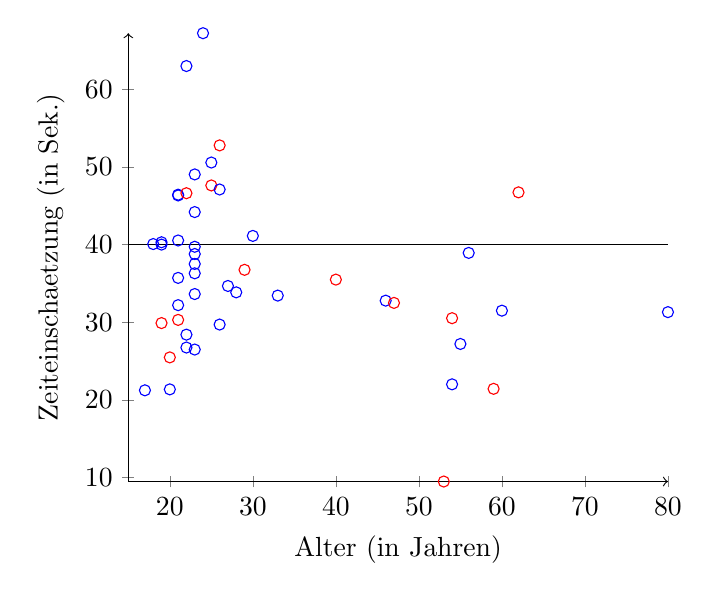
\begin{tikzpicture}
\begin{axis}[%
scatter/classes={%
    a={mark=o,draw=blue},
    b={mark=o,draw=red}},
    axis lines=middle,
    axis line style={->},
    x label style={at={(axis description cs:0.5,-0.1)},anchor=north},
    y label style={at={(axis description cs:-0.1,.5)},rotate=90,anchor=south},
    xlabel={Alter (in Jahren)},
    ylabel={Zeiteinschaetzung (in Sek.)}]
    % Orientierungslinie
	\addplot[domain=15:80]{40};
	% Scatter
    \addplot[scatter,only marks,%
    scatter src=explicit symbolic]%
table[meta=label] {
x y label
17 21.23 a
18 40.07 a
19 40.00 a
19 40.3 a
19 29.89 b
20 21.35 a
20 25.47 b
21 46.33 a
21 40.53 a
21 35.71 a
21 46.43 a
21 32.20 a
21 30.3 b
22 46.62 b
22 63.00 a
22 26.74 a
22 28.4 a
23 36.30 a
23 33.63 a
23 26.48 a
23 39.72 a
23 37.51 a
23 44.19 a
23 49.04 a
23 38.79 a
24 67.23 a
25 50.57 a
25 47.62 b
26 52.78 b
26 29.70 a
26 47.10 a
27 34.67 a
28 33.85 a
29 36.75 b
30 41.12 a
33 33.43 a
40 35.49 b
46 32.78 a
47 32.49 b
53 9.48 b
54 30.52 b
54 22 a
55 27.2 a
56 38.93 a
59 21.42 b
60 31.49 a
62 46.73 b	
80 31.3 a
	};
\end{axis}
\end{tikzpicture}
\caption{Zeiteinschätzung von 40 Sekunden ohne Gespräch nach Alter}
\label{Zeit40sek}
\end{minipage}
\hfill
\begin{minipage}[t]{0.49\linewidth}
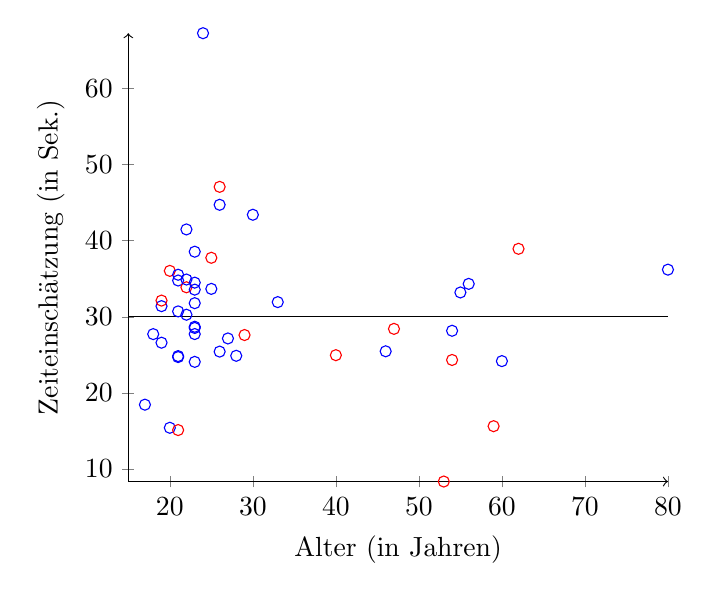
\begin{tikzpicture}
\begin{axis}[%
scatter/classes={%
    a={mark=o,draw=blue},
    b={mark=o,draw=red}},
    axis lines=middle,
    axis line style={->},
    x label style={at={(axis description cs:0.5,-0.1)},anchor=north},
    y label style={at={(axis description cs:-0.1,.5)},rotate=90,anchor=south},
    xlabel={Alter (in Jahren)},
    ylabel={Zeiteinschätzung (in Sek.)}]
    
    % Orientierungslinie
	\addplot[domain=15:80]{30};
	% Scatter
    \addplot[scatter,only marks,%
    scatter src=explicit symbolic]%
table[meta=label] {
x y label
17 18.44 a
18 27.72 a
19 26.59 a
19 31.4 a
19 32.13 b
20 15.40 a
20 36.04 b
21 34.77 a
21 35.53 a
21 24.83 a
21 30.71 a
21 24.70 a
21 15.1 b
22 33.88 b
22 41.49 a
22 30.27 a
22 34.9 a
23 28.69 a
23 34.49 a
23 24.07 a
23 31.79 a
23 27.73 a
23 28.53 a
23 33.57 a
23 38.56 a
24 67.30 a
25 33.67 a
25 37.76 b
26 47.09 b
26 25.42 a
26 44.73 a
27 27.15 a
28 24.87 a
29 27.60 b
30 43.42 a
33 31.93 a
40 24.95 b
46 25.46 a
47 28.41 b
53 8.33 b
54 24.32 b
54 28.16 a
55 33.2 a
56 34.33 a
59 15.61 b
60 24.17 a
62 38.94 b	
80 36.2 a
	};
\end{axis}
\end{tikzpicture}
\caption{Zeiteinschätzung von 30 Sekunden ohne Gespräch nach Alter}
\label{Zeit30sek}
\end{minipage}
\end{figure}

Die obigen Streudiagramme zeigen die ersten Zeiteinschätzungen ohne Gespräch in Relation zum Alter der Probanden. Der Großteil der Probanden ist unter 30 Jahre alt, dementsprechend sind für diese Alterskategorie die meisten Daten verfügbar.\\
In der Zeitspanne $+/-$ 10 Sekunden der angestrebten Zeit befinden sich die meisten der Probanden mit ihren Einschätzungen. Ebenfalls gibt es sowohl bei der 40- als auch bei der 30 Sekundeneinschätzung in nahezu jeder Alterskategorie Ausreißer, die sich stärker verschätzt haben. Aus diesen Diagrammen kann man schließen, dass es keine altersspezifischen Vor- oder Nachteile in einer Zeiteinschätzung gibt.



%%%%%%%%%%%%%%%%%%%%%%%%%%%%%%%%% HISTO ALTER %%%%%%%%%%%%%%%%%%%%%
\begin{figure}[H]
\begin{filecontents}{data.csv}
dist

21.23 
40.07 
40.00 
40.3 
29.89
21.35 
25.47
 46.33 
  40.53 
 35.71 
 46.43 
32.20 
 30.3 
 46.62 
 63.00 
 26.74 
 28.4 
 36.30 
 33.63 
 26.48 
 39.72 
37.51 
 44.19 
 49.04 
38.79 
 67.23 
 50.57 
47.62 
52.78 
 29.70 
 47.10 
 34.67 
33.85 
36.75 
 41.12 
 33.43 
 35.49 
 32.78 
 32.49
 9.48 
 30.52 
 22 
  27.2 
 38.93 
 21.42 
 31.49 
46.73 
 31.3 
\end{filecontents}
\begin{minipage}[t]{0.49\linewidth}
\begin{tikzpicture}
\begin{axis}[
    ybar,
    ymin=0
]
\addplot +[
    hist={
        bins=10,
        data min=0.5,
        data max=50
    }   
] table [y index=0] {data.csv};
\end{axis}
\end{tikzpicture}
\caption{Anzahl der Personen(y), welche die jeweilige Zeiteinschätzung(x) angaben - 40 Sekunden ohne Gespräch nach Alter.}
\label{HistZeit40sek}
\end{minipage}
\hfill
\begin{filecontents}{data.csv}
dist
 18.44 
 27.72 
 26.59 
 31.4 
 32.13 
 15.40 
 36.04 
 34.77 
 35.53 
 24.83 
 30.71 
 24.70 
 15.1 
 33.88 
 41.49 
 30.27 
 34.9 
 28.69 
 34.49 
 24.07 
 31.79 
 27.73 
 28.53 
 33.57 
 38.56
 67.30 
 33.67 
 37.76 
 47.09 
25.42 
44.73 
 27.15 
 24.87 
 27.60 
 43.42 
 31.93 
 24.95 
 25.46 
 28.41 
 8.33 
 24.32 
 28.16 
 33.2 
 34.33 
 15.61 
 24.17 
38.94 
 36.2 
\end{filecontents}
\begin{minipage}[t]{0.49\linewidth}
\begin{tikzpicture}
\begin{axis}[
    ybar,
    ymin=0
]
\addplot +[
    hist={
        bins=10,
        data min=0.5,
        data max=50
    }   
] table [y index=0] {data.csv};
\end{axis}
\end{tikzpicture}
\caption{Anzahl der Personen(y), welche die jeweilige Zeiteinschätzung(x) angaben - 30 Sekunden ohne Gespräch nach Alter.}
\label{HistZeit30sek}
\end{minipage}
\end{figure}

%%%%%%%%%%%%%%%%%%%%%%%%%%%%%%%%%%%%%%%%%%%%%%%%%%%%%%%% HISTO ALTER%%%%%%


%%%%%%%%%%%%%% SCATTERPLOT INTELLIGENZ
\begin{figure}[H]
\begin{minipage}[t]{0.49\linewidth}
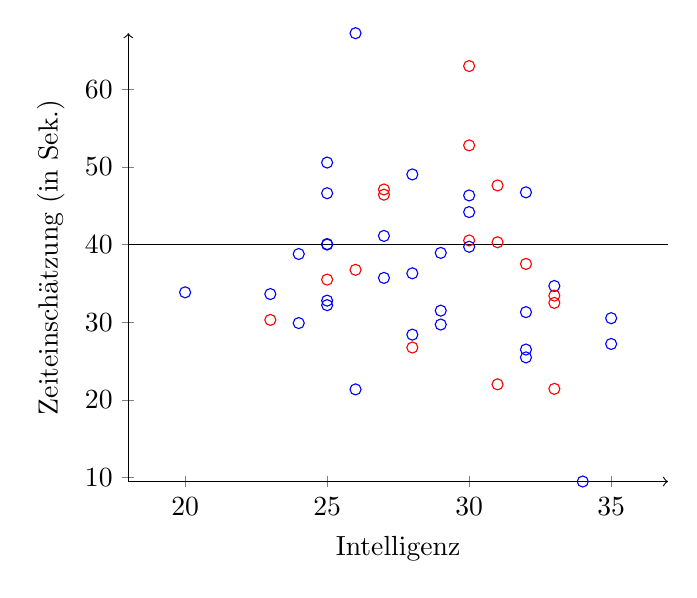
\begin{tikzpicture}
\begin{axis}[%
scatter/classes={%
    a={mark=o,draw=blue},
    b={mark=o,draw=red}},
    axis lines=middle,
    axis line style={->},
    x label style={at={(axis description cs:0.5,-0.1)},anchor=north},
    y label style={at={(axis description cs:-0.1,.5)},rotate=90,anchor=south},
    xlabel={Intelligenz},
    ylabel={Zeiteinschätzung (in Sek.)}]
  \addplot[domain=18:37]{40};
    \addplot[scatter,only marks,%
    scatter src=explicit symbolic]%
table[meta=label] {
x y label
20 33.85 a
23 30.3 b
23 33.63 a
24 29.89 a
24 38.79 a
25 40.07 a
25 40.00 a
25 32.20 a
25 46.62 a
25 50.57 a
25 35.49 b
25 32.78 a
26 21.35 a
26 67.23 a
26 36.75 b
27 35.71 a
27 46.43 b
27 47.10 b
27 41.12 a
28 26.74 b
28 28.4 a
28 36.30 a
28 49.04 a
29 29.70 a
29 38.93 a
29 31.49 a
30 46.33 a
30 40.53 b
30 63.00 b
30 39.72 a
30 44.19 a 
30 52.78 b
31 22 b
31 40.3 b
31 47.62 b
32 25.47 a
32 26.48 a
32 37.51 b
32 46.73 a
32 31.3 a
33 34.67 a
33 33.43 b
33 32.49 b
33 21.42 b
34 9.48 a
35 30.52 a
35 27.2 a 
    };
\end{axis}
\end{tikzpicture}
\caption{Zeiteinschätzung von 40 Sekunden ohne Gespräch nach Intelligenz}
\label{Zeit40sekInt}
\end{minipage}
\hfill
\begin{minipage}[t]{0.49\linewidth}
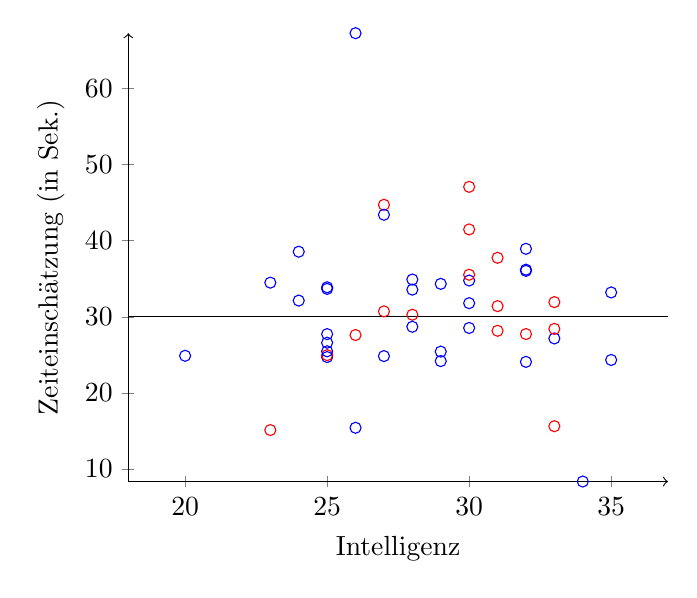
\begin{tikzpicture}
\begin{axis}[%
scatter/classes={%
    a={mark=o,draw=blue},
    b={mark=o,draw=red}},
    axis lines=middle,
    axis line style={->},
    x label style={at={(axis description cs:0.5,-0.1)},anchor=north},
    y label style={at={(axis description cs:-0.1,.5)},rotate=90,anchor=south},
    xlabel={Intelligenz},
    ylabel={Zeiteinschätzung (in Sek.)}]
    
    % Orientierungslinie
	\addplot[domain=18:37]{30};
	% Scatter
    \addplot[scatter,only marks,%
    scatter src=explicit symbolic]%
table[meta=label] {
x y label
20 24.87 a
23 15.1 b
23 34.49 a
24 32.13 a
24 38.56 a
25 27.72 a
25 26.59 a
25 24.70 a
25 33.88 a
25 33.67 a
25 24.95 b
25 25.46 a
26 15.40 a
26 67.30 a
26 27.60 b
27 24.83 a
27 30.71 b
27 44.73 b
27 43.42 a
28 30.27 b
28 34.9 a
28 28.69 a
28 33.57 a
29 25.42 a
29 34.33 a
29 24.17 a
30 34.77 a
30 35.53 b
30 41.49 b
30 31.79 a
30 28.53 a 
30 47.09 b
31 28.16 b
31 31.4 b
31 37.76 b
32 36.04 a
32 24.07 a
32 27.73 b
32 38.94 a
32 36.2 a
33 27.15 a
33 31.93 b
33 28.41 b
33 15.61 b
34 8.33 a
35 24.32 a
35 33.2 a 
    };
    \end{axis}
\end{tikzpicture}
\caption{Zeiteinschätzung von 30 Sekunden ohne Gespräch nach Intelligenz}
\label{Zeit30sekInt}
\end{minipage}
\end{figure}

Der benutzte Intelligenztest hat eine Höchstpunktzahl von 37 Punkten und sieht folgende Verteilung vor: 0-5 Punkte (sehr niedrige Intelligenz), 6-20 Punkte (niedrige Intelligenz), 21-30 Punkte (durchschnittliche Intelligenz), 31-33 Punkte (hohe Intelligenz), 34-37 Punkte (sehr hohe Intelligenz).
Sortiert man die Daten nach Intelligenz, fällt bei der normalen Zeiteinschätzung auf, dass die gemessenen Werte auch hier relativ gleichmäßig verteilt sind. Es gibt zwei besonders starke Ausreißer in der durchschnittlichen und höheren Intelligenz, aber ähnlich wie in der Altersverteilung befinden sich die meisten Werte $+/-$10 Sekunden vom erwünschten Wert.

%%%%%%%%%%%%%%%%%%%%%%%%%%%%%%%%% HISTO intelligenz %%%%%%%%%%%%%%%%%%%%%
\begin{figure}[H]
\begin{filecontents}{data.csv}
dist

 33.85 
 30.3 
 33.63 
 29.89 
 38.79 
 40.07 
 40.00 
 32.20 
 46.62 
 50.57 
 35.49 
 32.78 
 21.35 
 67.23 
 36.75 
 35.71
 46.43 
 47.10 
 41.12 
 26.74 
 28.4 
 36.30 
 49.04 
 29.70 
 38.93 
 31.49 
 46.33 
 40.53 
63.00 
 39.72 
 44.19 
 52.78 
 22 
 40.3 
 47.62 
 25.47 
 26.48 
 37.51 
 46.73 
 31.3 
 34.67 
 33.43 
 32.49 
 21.42 
 9.48 
 30.52 
 27.2 
\end{filecontents}
\begin{minipage}[t]{0.49\linewidth}
\begin{tikzpicture}
\begin{axis}[
    ybar,
    ymin=0
]
\addplot +[
    hist={
        bins=10,
        data min=0.5,
        data max=50
    }   
] table [y index=0] {data.csv};
\end{axis}
\end{tikzpicture}
\caption{Anzahl der Personen(y), welche die jeweilige Zeiteinschätzung(x) angaben - 40 Sekunden ohne Gespräch nach Intelligenz.}
\label{HistZeit40sekInt}
\end{minipage}
\hfill
\begin{filecontents}{data.csv}
dist
  24.87 
 15.1 
 34.49 
 32.13 
 38.56 
 27.72 
 26.59 
 24.70 
 33.88
 33.67 
 24.95 
 25.46 
 15.40 
 67.30 
 27.60 
 24.83 
 30.71 
 44.73 
 43.42 
 30.27 
 34.9 
 28.69 
 33.57 
 25.42 
 34.33 
 24.17 
 34.77 
 35.53 
 41.49 
 31.79 
 28.53 
 47.09 
 28.16 
 31.4 
 37.76 
 36.04 
 24.07 
 27.73 
 38.94 
 36.2 
 27.15 
 31.93 
 28.41 
 15.61 
 8.33 
 24.32 
33.2 
\end{filecontents}
\begin{minipage}[t]{0.49\linewidth}
\begin{tikzpicture}
\begin{axis}[
    ybar,
    ymin=0
]
\addplot +[
    hist={
        bins=10,
        data min=0.5,
        data max=50
    }   
] table [y index=0] {data.csv};
\end{axis}
\end{tikzpicture}
\caption{Anzahl der Personen(y), welche die jeweilige Zeiteinschätzung(x) angaben - 30 Sekunden ohne Gespräch nach Intelligenz.}
\label{HistZeit30sekInt}
\end{minipage}
\end{figure}

%%%%%%%%%%%%%%%%%%%%%%%%%%%%%%%%%%%%%%%%%%%%%%%%%%%%%%%% HISTO Intelligenz %%%%%%
%%%%%%%%%%%%%% SCATTERPLOTS NACH TEMPERATUR
\begin{figure}[H]
\begin{minipage}[t]{0.49\linewidth}
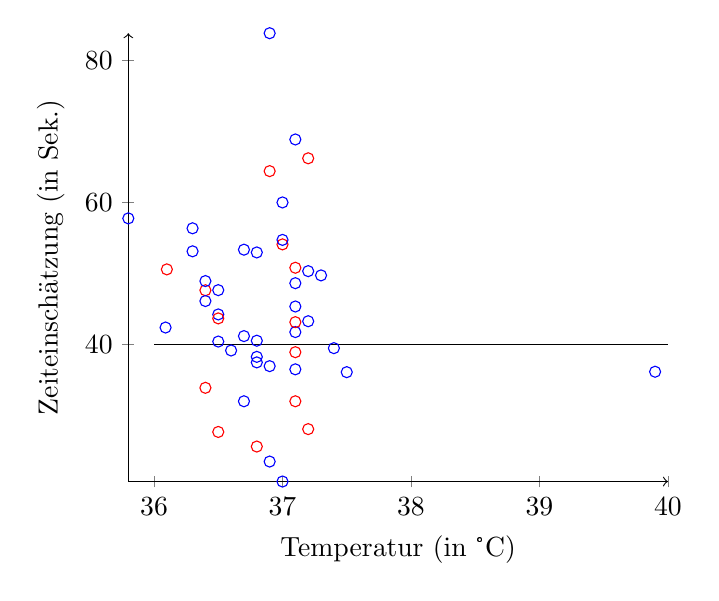
\begin{tikzpicture}
\begin{axis}[%
scatter/classes={%
    a={mark=o,draw=blue},
    b={mark=o,draw=red}},
    axis lines=middle,
    axis line style={->},
    x label style={at={(axis description cs:0.5,-0.1)},anchor=north},
    y label style={at={(axis description cs:-0.1,.5)},rotate=90,anchor=south},
    xlabel={Temperatur (in °C)},
    ylabel={Zeiteinschätzung (in Sek.)}]
     \addplot[domain=36:40]{39.9};
    \addplot[scatter,only marks,%
    scatter src=explicit symbolic]%
table[meta=label] {
x y label
35.8 57.75 a
36.09 42.34 a
36.1 50.55 b
36.3 53.1 a
36.3 56.35 a
36.4 47.6 b
36.4 46.08 a
36.4 48.9 a
36.4 33.83 b
36.5 27.6 b
36.5 44.19 a
36.5 43.63 b
36.5 40.36 a
36.5 47.62 a
36.6 39.1 a
36.7 53.33 a
36.7 41.13 a
36.7 31.93 a
36.8 40.48 a
36.8 52.94 a
36.8 25.54 b	
36.8 38.2 a
36.8 37.42 a
36.9 23.42 a
36.9 64.42 b
36.9 83.89 a
36.9 36.89 a
37.00 20.6 a
37.00 60 a
37.00 54.08  b
37.00 54.71 a
37.1 38.86 b
37.1 41.7 a
37.1 45.31 a
37.1 68.89 a
37.1 36.44 a
37.1 43.1 b
37.1 50.78 b
37.1 31.93 b
37.1 48.6 a
37.2 66.23 b
37.2 43.23 a
37.2 28 b
37.2 50.3 a
37.3 49.7 a
37.4 39.43 a 
37.5 36.04 a
39.9 36.1 a 
    };
\end{axis}
\end{tikzpicture}
\caption{Zeiteinschätzung von 40 Sekunden ohne Gespräch nach Temperatur}
\label{Zeit40sekTemp}
\end{minipage}
\hfill
\begin{minipage}[t]{0.49\linewidth}
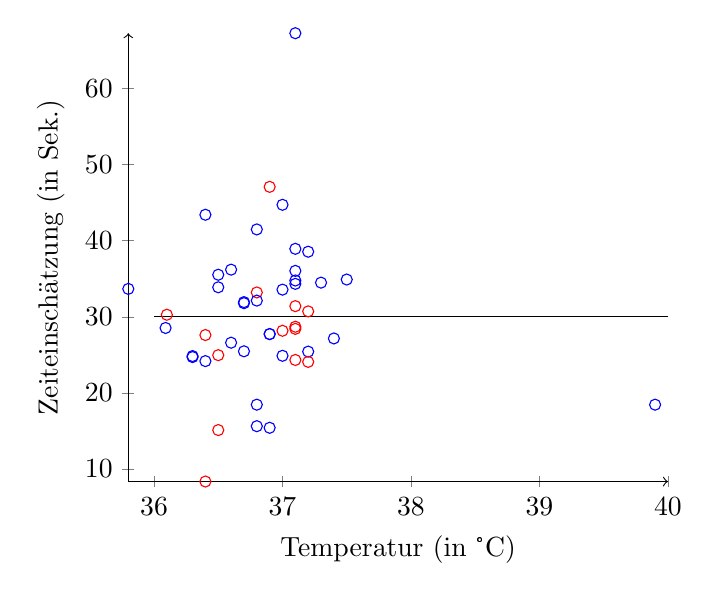
\begin{tikzpicture}
\begin{axis}[%
scatter/classes={%
    a={mark=o,draw=blue},
    b={mark=o,draw=red}},
    axis lines=middle,
    axis line style={->},
    x label style={at={(axis description cs:0.5,-0.1)},anchor=north},
    y label style={at={(axis description cs:-0.1,.5)},rotate=90,anchor=south},
    xlabel={Temperatur (in °C)},
    ylabel={Zeiteinschätzung (in Sek.)}]
    % Orientierungslinie
	\addplot[domain=36:40]{30};
	% Scatter
    \addplot[scatter,only marks,%
    scatter src=explicit symbolic]%
table[meta=label] {
x y label
35.8 33.67 a
36.09 28.53 a
36.1 30.27 b
36.3 24.70 a
36.3 24.83 a
36.4 27.60 b
36.4 43.42 a
36.4 24.17 a
36.4 8.33 b
36.5 15.1 b
36.5 33.88 a
36.5 24.95 b
36.5 35.53 a
36.6 36.2 a
36.6 26.59 a
36.7 31.79 a
36.7 31.93 a
36.7 25.46 a
36.8 41.49 a
36.8 15.61 a
36.8 33.2 b
36.8 18.44 a
36.8 32.13 a
36.9 27.72 a
36.9 47.09 b
36.9 27.73 a
36.9 15.40 a
37.00 44.73 a
37.00 33.57 a
37.00 28.16  b
37.00 24.87 a
37.1 28.69 b
37.1 34.33 a
37.1 34.77 a
37.1 36.04 a
37.1 38.94 a
37.1 28.41 b
37.1 24.32 b
37.1 31.4 b
37.1 67.30 a
37.2 30.71 b
37.2 25.42 a
37.2 24.07 b
37.2 38.56 a
37.3 34.49 a
37.4 27.15 a 
37.5 34.9 a
39.9 18.44 a 
	};
\end{axis}
\end{tikzpicture}
\caption{Zeiteinschätzung von 30 Sekunden ohne Gespräch nach Temperatur}
\label{Zeit30sekTemp}
\end{minipage}
\end{figure}

Die meisten der Probanden hatten eine durchschnittliche Körpertemperatur, lediglich einer lag mit 39,9°C über dem Durchschnitt. Auffällig ist, dass es die meisten Abweichungen im direkten Umfeld von 37°C gab, bei niedrigerer Temperatur nähern sich die Zeiteinschätzungen dem gewünschten Ergebnis etwas mehr an. Auch der Proband mit der sehr hohen Temperatur lag in einer Schätzung recht nah am gewünschten Ergebnis und in der anderen Schätzung immernoch in der normalen Abweichung.
%%%%%%%%%%%%%%%%%%%%%%%%%%%%%%%%% HISTO TEMP %%%%%%%%%%%%%%%%%%%%%
\begin{figure}[H]
\begin{filecontents}{data.csv}
dist
  57.75 
 42.34 
 50.55 
 53.1 
 56.35 
 47.6 
 46.08 
 48.9 
 33.83 
 27.6 
 44.19 
 43.63 
 40.36 
 47.62 
 39.1 
 53.33 
 41.13 
 31.93 
 40.48 
 52.94 
25.54 
 38.2 
37.42 
23.42 
 64.42 
 83.89 
36.89 
20.6 
 60 
 54.08  
 54.71 
 38.86 
 41.7 
 45.31 
 68.89 
36.44 
 43.1 
50.78 
31.93 
48.6 
66.23 
 43.23 
 28 
 50.3 
 49.7
 39.43 
 36.04 
36.1 
\end{filecontents}
\begin{minipage}[t]{0.49\linewidth}
\begin{tikzpicture}
\begin{axis}[
    ybar,
    ymin=0
]
\addplot +[
    hist={
        bins=10,
        data min=0.5,
        data max=50
    }   
] table [y index=0] {data.csv};
\end{axis}
\end{tikzpicture}
\caption{Anzahl der Personen(y), welche die jeweilige Zeiteinschätzung(x) angaben - 40 Sekunden ohne Gespräch nach Temperatur.}
\label{HistZeit40sekTemp}
\end{minipage}
\hfill
\begin{filecontents}{data.csv}
dist
  33.67 
 28.53 
 30.27 
 24.70 
 24.83 
 27.60 
 43.42 
 24.17 
 8.33 
 15.1 
 33.88 
 24.95 
 35.53 
 36.2 
 26.59 
 31.79
 31.93 
 25.46 
 41.49 
 15.61 
 33.2
 18.44 
 32.13 
 27.72 
 47.09 
 27.73 
 15.40 
 44.73 
 33.57 
 28.16  
 24.87 
 28.69 
 34.33 
 34.77 
 36.04 
 38.94 
 28.41 
 24.32 
 31.4 
 67.30 
 30.71 
 25.42 
 24.07 
 38.56 
 34.49 
 27.15  
 34.9 
18.44 
\end{filecontents}
\begin{minipage}[t]{0.49\linewidth}
\begin{tikzpicture}
\begin{axis}[
    ybar,
    ymin=0
]
\addplot +[
    hist={
        bins=10,
        data min=0.5,
        data max=50
    }   
] table [y index=0] {data.csv};
\end{axis}
\end{tikzpicture}
\caption{Anzahl der Personen(y), welche die jeweilige Zeiteinschätzung(x) angaben - 30 Sekunden ohne Gespräch nach Temparatur.}
\label{HistZeit30sekTemp}
\end{minipage}
\end{figure}

%%%%%%%%%%%%%%%%%%%%%%%%%%%%%%%%%%%%%%%%%%%%%%%%%%%%%%%% HISTO TEMP %%%%%%
%%%%%%%%%%%%%%%%%%% 
\begin{figure}[H]
\begin{minipage}[t]{0.49\linewidth}
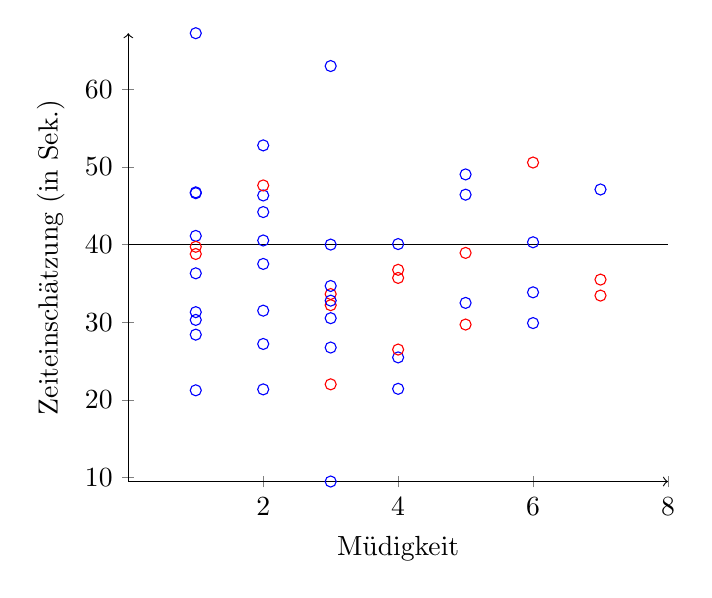
\begin{tikzpicture}
\begin{axis}[%
scatter/classes={%
    a={mark=o,draw=blue},
    b={mark=o,draw=red}},
    axis lines=middle,
    axis line style={->},
    x label style={at={(axis description cs:0.5,-0.1)},anchor=north},
    y label style={at={(axis description cs:-0.1,.5)},rotate=90,anchor=south},
    xlabel={Müdigkeit},
    ylabel={Zeiteinschätzung (in Sek.)}]
    \addplot[domain=0:8]{40};
    \addplot[scatter,only marks,%
    scatter src=explicit symbolic]%
table[meta=label] {
x y label
1 30.3 a
1 38.79 b
1 46.62 a
1 67.23 a
1 41.12 a
1 28.4 a
1 36.30 a
1 39.72 b
1 46.73 a
1 31.3 a
1 21.23 a
2 21.35 a
2 31.49 a
2 46.33 a
2 40.53 a
2 47.62 b
2 44.19 a
2 52.78 a
2 37.51 a
2 27.2 a
3 33.63 b
3 40.00 a
3 32.20 b
3 32.78 a
3 26.74 a
3 63.00 a
3 22 b
3 34.67 a
3 9.48 a
3 30.52 a
4 40.07 a
4 36.75 b
4 35.71 b
4 25.47 a
4 26.48 b
4 21.42 a
5 46.43 a
5 49.04 a
5 29.70 b
5 38.93 b
5 32.49 a
6 40.3 a
6 33.85 a
6 29.89 a
6 50.57 b
7 35.49 b
7 47.10 a
7 33.43 b
    };
\end{axis}
\end{tikzpicture}
\caption{Zeiteinschätzung von 40 Sekunden ohne Gespräch nach Müdigkeit}
\label{Zeit40sekMued}
\end{minipage}
\hfill
\begin{minipage}[t]{0.49\linewidth}
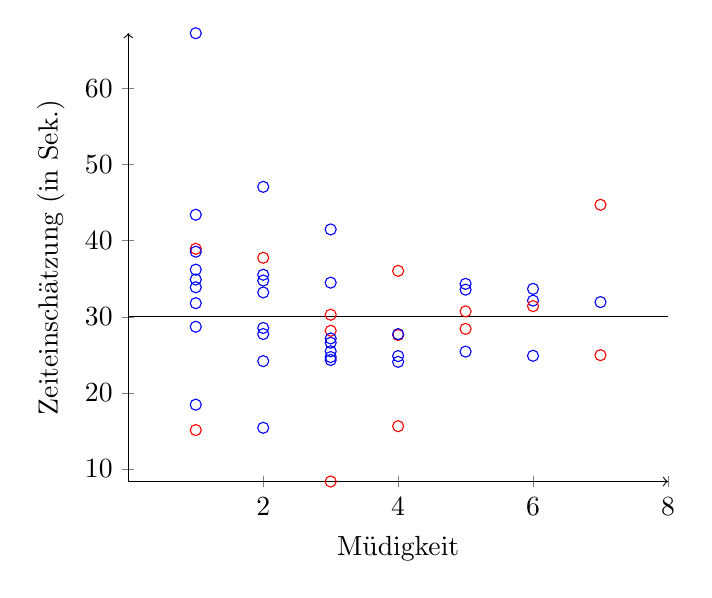
\begin{tikzpicture}
\begin{axis}[%
scatter/classes={%
    a={mark=o,draw=blue},
    b={mark=o,draw=red}},
    axis lines=middle,
    axis line style={->},
    x label style={at={(axis description cs:0.5,-0.1)},anchor=north},
    y label style={at={(axis description cs:-0.1,.5)},rotate=90,anchor=south},
    xlabel={Müdigkeit},
    ylabel={Zeiteinschätzung (in Sek.)}]
    % Orientierungslinie
	\addplot[domain=0:8]{30};
	% Scatter
    \addplot[scatter,only marks,%
    scatter src=explicit symbolic]%
table[meta=label] {
x y label
1 43.42 a
1 15.1 b
1 33.88 a
1 36.2 a
1 31.79 a
1 18.44 a
1 28.69 a
1 38.94 b
1 67.30 a
1 38.56 a
1 34.9 a
2 28.53 a
2 24.17 a
2 35.53 a
2 37.76 b
2 33.2 a
2 47.09 a
2 27.73 a
2 15.40 a
2 34.77 a
3 30.27 b
3 24.70 a
3 8.33 b
3 26.59 a
3 25.46 a
3 41.49 a
3 28.16 b
3 24.32 a
3 34.49 a
3 27.15 a
4 24.83 a
4 27.60 b
4 15.61 b
4 27.72 a
4 36.04 b
4 24.07 a
5 33.57 a
5 34.33 a
5 28.41 b
5 30.71 b
5 25.42 a
6 33.67 a
6 32.13 a
6 24.87 a
6 31.4 b
7 24.95 b
7 31.93 a
7 44.73 b
	};
\end{axis}
\end{tikzpicture}	
\caption{Zeiteinschätzung von 30 Sekunden ohne Gespräch nach Müdigkeit}
\label{Zeit30sekMued}
\end{minipage}
\end{figure}

Die Müdigkeitsskala erstreckt sich von 1 (nicht müde) bis 10 (sehr müde).\\
Die meisten Versuchspersonen waren wenig bis durchschnittlich müde, haben aber nicht besser geschätzt als jene, die angaben, überdurchschnittlich müde zu sein. Allerdings muss man hier beachten, dass wir nur wenige Versuchspersonen, die sehr müde waren und entsprechend weniger aussagekräftige Daten.
Auch hier sind die gemessenen Werte wieder recht weit gestreut.
\linebreak
\linebreak
%%%%%%%%%%%%%%%%%%%%%%%%%%%%%%%%% HISTO MÜDE %%%%%%%%%%%%%%%%%%%%%
\begin{figure}[H]
\begin{filecontents}{data.csv}
dist
   30.3 
   38.79 
 46.62 
 67.23 
 41.12 
 28.4 
 36.30 
 39.72 
 46.73 
 31.3 
 21.23 
 21.35 
 31.49 
 46.33 
 40.53 
 47.62 
 44.19 
 52.78 
 37.51 
 27.2 
 33.63 
 40.00 
 32.20 
 32.78 
 26.74 
 63.00 
 22 
 34.67 
 9.48 
 30.52 
 40.07 
 36.75 
 35.71 
 25.47 
 26.48 
 21.42 
 46.43 
 49.04 
 29.70 
 38.93 
 32.49 
 40.3 
 33.85 
 29.89 
 50.57 
 35.49 
 47.10 
 33.43 
\end{filecontents}
\begin{minipage}[t]{0.49\linewidth}
\begin{tikzpicture}
\begin{axis}[
    ybar,
    ymin=0
]
\addplot +[
    hist={
        bins=10,
        data min=0.5,
        data max=50
    }   
] table [y index=0] {data.csv};
\end{axis}
\end{tikzpicture}
\caption{Anzahl der Personen(y), welche die jeweilige Zeiteinschätzung(x) angaben - 40 Sekunden ohne Gespräch nach Müdigkeit.}
\label{HistZeit40sekMued}
\end{minipage}
\hfill
\begin{filecontents}{data.csv}
dist
  33.67 
 28.53 
 30.27 
 24.70 
 24.83 
 27.60 
 43.42 
 24.17 
 8.33 
 15.1 
 33.88 
 24.95 
 35.53 
 36.2 
 26.59 
 31.79
 31.93 
 25.46 
 41.49 
 15.61 
 33.2
 18.44 
 32.13 
 27.72 
 47.09 
 27.73 
 15.40 
 44.73 
 33.57 
 28.16  
 24.87 
 28.69 
 34.33 
 34.77 
 36.04 
 38.94 
 28.41 
 24.32 
 31.4 
 67.30 
 30.71 
 25.42 
 24.07 
 38.56 
 34.49 
 27.15  
 34.9 
18.44 
\end{filecontents}
\begin{minipage}[t]{0.49\linewidth}
\begin{tikzpicture}
\begin{axis}[
    ybar,
    ymin=0
]
\addplot +[
    hist={
        bins=10,
        data min=0.5,
        data max=50
    }   
] table [y index=0] {data.csv};
\end{axis}
\end{tikzpicture}
\caption{Anzahl der Personen(y), welche die jeweilige Zeiteinschätzung(x) angaben - 30 Sekunden ohne Gespräch nach Müdigkeit.}
\label{HistZeit30sekMued}
\end{minipage}
\end{figure}

%%%%%%%%%%%%%%%%%%%%%%%%%%%%%%%%%%%%%%%%%%%%%%%%%%%%%%%% HISTO MÜDE %%%%%%
%%%%%%%%%%%%%%%%%%%
%%%%%%%%%%%%%%%%%%%%%%%%%%%%%%%%%%%%%%%%%%%%%%%%%%%%%%%%%%%%%%%%%%%%%%%%%%%%%%%%%%%%%%%%%




%%%% SCATTERPLOTS MIT GESRPÄCH
%%%%%%%%%%%%%%%%%%%%%%%%%%%%%%%%%%%%%%%%%%%%%%%%%%%%%%%%%%%%%%%%%%%%%%%%%%%%%%%%%%%%%%%%%
% SCATTERPLOT ALTER

%%%%%%%%%%%%%%%%%%%%%%%%%%%%%%%%% HISTO alter %%%%%%%%%%%%%%%%%%%%%
\begin{figure}[H]
\begin{minipage}[t]{0.49\linewidth}
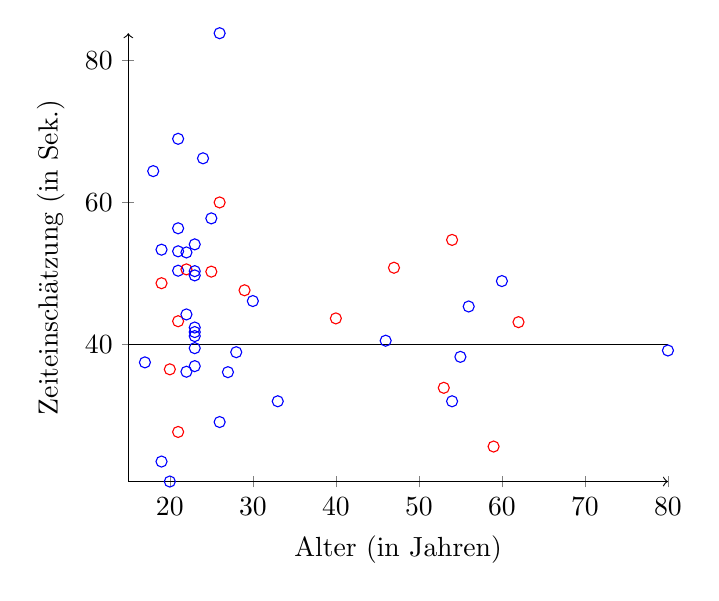
\begin{tikzpicture}
\begin{axis}[%
scatter/classes={%
    a={mark=o,draw=blue},
    b={mark=o,draw=red}},
    axis lines=middle,
    axis line style={->},
    x label style={at={(axis description cs:0.5,-0.1)},anchor=north},
    y label style={at={(axis description cs:-0.1,.5)},rotate=90,anchor=south},
    xlabel={Alter (in Jahren)},
    ylabel={Zeiteinschätzung (in Sek.)}]
    % Orientierungslinie
	\addplot[domain=15:80]{40};
	% Scatter
    \addplot[scatter,only marks,%
    scatter src=explicit symbolic]%
table[meta=label] {
x y label
17 37.42 a
18 64.42 a
19 53.33 a
19 23.42 a
19 48.6 b
20 20.6 a
20 36.44 b
21 53.1 a
21 56.35 a
21 27.6 b
21 50.36 a
21 68.98 a
21 43.23 b
22 50.55 b
22 44.19 a
22 52.94 a
22 36.1 a
23 54.08 a
23 42.34 a
23 41.13 a
23 36.89 a
23 41.7 a
23 50.3 a
23 49.7 a
23 39.43 a
24 66.23 a
25 50.23 b
25 57.75 a
26 60 b
26 83.89 a
26 29.00 a
27 36.04 a
28 38.86 a
29 47.6 b
30 46.08 a
33 31.93 a
40 43.63 b
46 40.48 a
47 50.78 b
53 33.83 b
54 54.71 b
54 31.93 a
55 38.2 a
56 45.31 a
59 25.54 b
60 48.9 a
62 43.1 b	
80 39.1 a
	};
\end{axis}
\end{tikzpicture}
\caption{Zeiteinschätzung von 40 Sekunden mit Gespräch nach Alter}
\label{Zeit40sekAltMitGespr}
\end{minipage}
\hfill
\begin{filecontents}{data.csv}
dist
 42.34 
 41.13 
 36.89 
 41.7 
 50.3 
 49.7 
 39.43 
 66.23 
 50.23 
 57.75 
 60 
 83.89 
 29.00 
 36.04 
 38.86 
 47.6 
 46.08 
 31.93 
 43.63 
 40.48 
 50.78 
 33.83 
 54.71 
 31.93 
 38.2 
 45.31 
 25.54
 48.9 
 43.1	
 39.1 
\end{filecontents}
\begin{minipage}[t]{0.49\linewidth}
\begin{tikzpicture}
\begin{axis}[
    ybar,
    ymin=0
]
\addplot +[
    hist={
        bins=10,
        data min=0.5,
        data max=50
    }   
] table [y index=0] {data.csv};
\end{axis}
\end{tikzpicture}
\caption{Anzahl der Personen(y), welche die jeweilige Zeiteinschätzung(x) angaben - 40 Sekunden mit Gespräch nach Alter.}
\label{Zeit40sekAlt}
\end{minipage}
\end{figure}

Es ist auffällig, dass viele der jüngeren Versuchspersonen die Zeit im Gespräch unterschätzten. Nichtsdestoweniger lagen aber auch viele der Versuchspersonen immernoch recht nah am gefragten Wert und das aus allen Altersklassen.
%%%%%%%%%%%%%%%%%%%%%%%%%%%%%%%%%%%%%%%%%%%%%%%%%%%%%%%%%%%%%%%%%%%%%%%%%%%%%%%%%%
\begin{figure}[H]
\begin{minipage}[t]{0.49\linewidth}
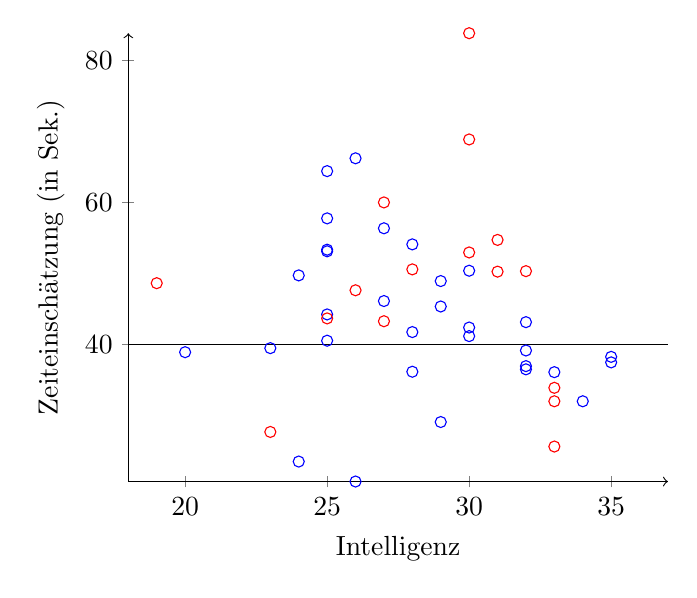
\begin{tikzpicture}
\begin{axis}[%
scatter/classes={%
    a={mark=o,draw=blue},
    b={mark=o,draw=red}},
    axis lines=middle,
    axis line style={->},
    x label style={at={(axis description cs:0.5,-0.1)},anchor=north},
    y label style={at={(axis description cs:-0.1,.5)},rotate=90,anchor=south},
    xlabel={Intelligenz},
    ylabel={Zeiteinschätzung (in Sek.)}]
  \addplot[domain=18:37]{40};
    \addplot[scatter,only marks,%
    scatter src=explicit symbolic]%
table[meta=label] {
x y label
19 48.6 b
20 38.86 a
23 27.6 b
23 39.43 a
24 23.42 a
24 49.7 a
25 64.42 a
25 53.33 a
25 53.1 a
25 44.19 a
25 57.75 a
25 43.63 b
25 40.48 a
26 20.6 a
26 66.23 a
26 47.6 b
27 56.35 a
27 43.23 b
27 60 b
27 46.08 a
28 50.55 b
28 36.1 a
28 54.08 a
28 41.7 a
29 29 a
29 45.31 a
29 48.9 a
30 50.36 a
30 68.89 b
30 52.94 b
30 42.34 a
30 41.13 a 
30 83.89 b
31 54.71 b
31 50.23 b
32 36.44 a
32 36.89 a
32 50.3 b
32 43.1 a
32 39.1 a
33 36.04 a
33 31.93 b
33 25.54 b
33 33.83 b
34 31.93 a
35 38.2 a
35 37.42 a 
	};
\end{axis}
\end{tikzpicture}
\caption{Zeiteinschätzung von 40 Sekunden mit Gespräch nach Intelligenz}
\label{Zeit40sekGesprInt}
\end{minipage}
\hfill
\begin{filecontents}{data.csv}
dist
  48.6 
 38.86 
 27.6 
 39.43 
 23.42 
 49.7 
 64.42 
 53.33 
 53.1 
 44.19 
 57.75 
 43.63 
 40.48 
 20.6 
 66.23 
 47.6 
 56.35 
 43.23 
 60 
 46.08 
 50.55 
 36.1 
 54.08 
 41.7 
 29 
 45.31 
 48.9 
 50.36 
 68.89 
 52.94 
 42.34 
 41.13 
 83.89 
 54.71 
 50.23 
 36.44 
 36.89 
 50.3 
 43.1 
 39.1 
 36.04 
 31.93 
 25.54 
 33.83 
 31.93 
 38.2 
 37.42 
\end{filecontents}
\begin{minipage}[t]{0.49\linewidth}
\begin{tikzpicture}
\begin{axis}[
    ybar,
    ymin=0
]
\addplot +[
    hist={
        bins=10,
        data min=0.5,
        data max=50
    }   
] table [y index=0] {data.csv};
\end{axis}
\end{tikzpicture}
\caption{Anzahl der Personen(y), welche die jeweilige Zeiteinschätzung(x) angaben - 40 Sekunden mit Gespräch nach Intelligenz.}
\label{HistZeit40sekGesprInt}
\end{minipage}
\end{figure}

Viele der durchschnittlich intelligenten Versuchspersonen schätzen die tatsächlich verstrichene Zeit als kürzer ein, wohingegen die Teilnehmer mit niedrigerer und höherer Intelligenz näher am Idealwert liegen. Hierbei sei wieder angemerkt, dass die meisten Versuchspersonen im Mittelwert liegen und nur eine Minderheit die Extreme auf beiden Seiten darstellen.

%%%%%%%%%%%%%%%%%%%%%%%%%%%%%%%%%%%%%%%%%%%%%%%%%%%%%%%%%%%%%%%%%%%%%%%%%%%%%%%%%%%%%
\begin{figure}[H]
\begin{minipage}[t]{0.49\linewidth}
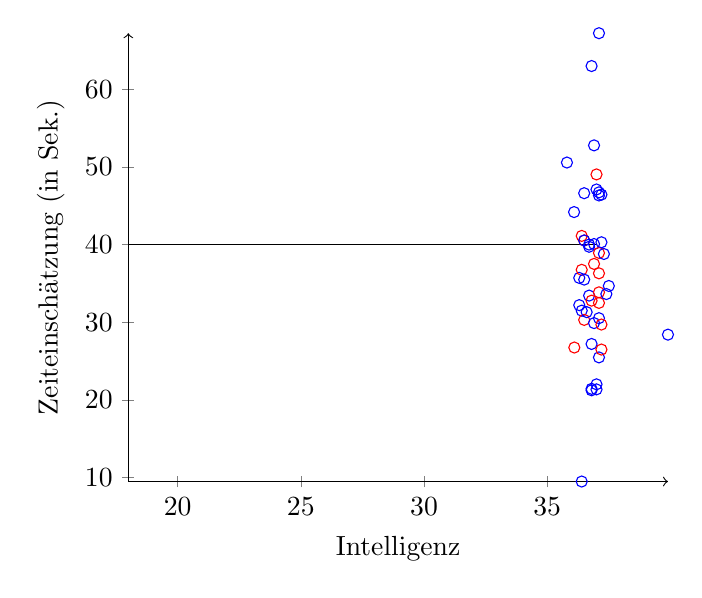
\begin{tikzpicture}
\begin{axis}[%
scatter/classes={%
    a={mark=o,draw=blue},
    b={mark=o,draw=red}},
    axis lines=middle,
    axis line style={->},
    x label style={at={(axis description cs:0.5,-0.1)},anchor=north},
    y label style={at={(axis description cs:-0.1,.5)},rotate=90,anchor=south},
    xlabel={Intelligenz},
    ylabel={Zeiteinschätzung (in Sek.)}]
  \addplot[domain=18:37]{40};
    \addplot[scatter,only marks,%
    scatter src=explicit symbolic]%
table[meta=label] {
x y label
35.8 50.57 a
36.09 44.19 a
36.1 26.74 b
36.3 32.2 a
36.3 35.71 a
36.4 41.12 b
36.4 31.49 a
36.4 9.48 a
36.4 36.75 b
36.5 30.3 b
36.5 46.62 a
36.5 40.53 b
36.5 40.53 a
36.5 35.49 a
36.6 31.3 a
36.7 39.72 a
36.7 40.00 a
36.7 33.43 a
36.8 21.23 a
36.8 27.2 a
36.8 32.78 b
36.8 63.00 a
36.8 21.42 a
36.9 52.78 a
36.9 37.51 b
36.9 40.07 a
36.9 29.89 a
37.00 21.35 a
37.00 22 a
37.00 49.04  b
37.00 47.1 a
37.1 36.3 b
37.1 46.73 a
37.1 46.33 a
37.1 30.52 a
37.1 25.47 a
37.1 38.93 b
37.1 32.49 b
37.1 33.85 b
37.1 67.23 a
37.2 26.48 b
37.2 46.43 a
37.2 29.7 b
37.2 40.3 a
37.3 38.79 a
37.4 33.63 a 
37.5 34.67 a
39.9 28.4 a 
	};
\end{axis}
\end{tikzpicture}
\caption{Zeiteinschätzung von 40 Sekunden mit Gespräch nach Temperatur}
\label{Zeit40sekGesprTemp}
\end{minipage}
\hfill
\begin{filecontents}{data.csv}
dist
   50.57 
 44.19 
 26.74 
 32.2 
 35.71 
 41.12 
 31.49 
 9.48 
 36.75 
 30.3 
 46.62 
 40.53 
 40.53 
 35.49 
 31.3 
 39.72 
 40.00 
 33.43 
 21.23 
 27.2 
 32.78 
 63.00 
 21.42 
52.78 
37.51 
 40.07 
 29.89 
 21.35 
 22 
 49.04  
 47.1 
 36.3 
 46.73 
 46.33 
 30.52 
 25.47 
 38.93 
32.49
 33.85 
 67.23 
 26.48 
 46.43 
 29.7 
 40.3 
 38.79 
 33.63  
 34.67 
28.4 
\end{filecontents}
\begin{minipage}[t]{0.49\linewidth}
\begin{tikzpicture}
\begin{axis}[
    ybar,
    ymin=0
]
\addplot +[
    hist={
        bins=10,
        data min=0.5,
        data max=50
    }   
] table [y index=0] {data.csv};
\end{axis}
\end{tikzpicture}
\caption{Anzahl der Personen(y), welche die jeweilige Zeiteinschätzung(x) angaben - 40 Sekunden mit Gespräch nach Temperatur.}
\label{HistZeit40sekGesprTemp}
\end{minipage}
\end{figure}
Ähnlich wie bei den Einschätzungen ohne Gespräch befinden sich hier die stärksten Abweichungen bei den Versuchspersonen mit einer Temperatur knapp um 37°C. Bei Versuchspersonen mit niedrigerer Temperatur gibt es ebenfalls, wenn auch nicht so starke, Abweichungen. Die Person mit der hohen Körpertemperatur liegt nah am Idealwert.



%%%%%%%%%%%%%%%%%%%%%%%%%%%%%%%%%%%%%%%%%%%%%%%%%%%%%%%%%%%%%%%%%%%%%%%%%%%%%%%%%%%%%

\begin{figure}[H]
\begin{minipage}[t]{0.49\linewidth}
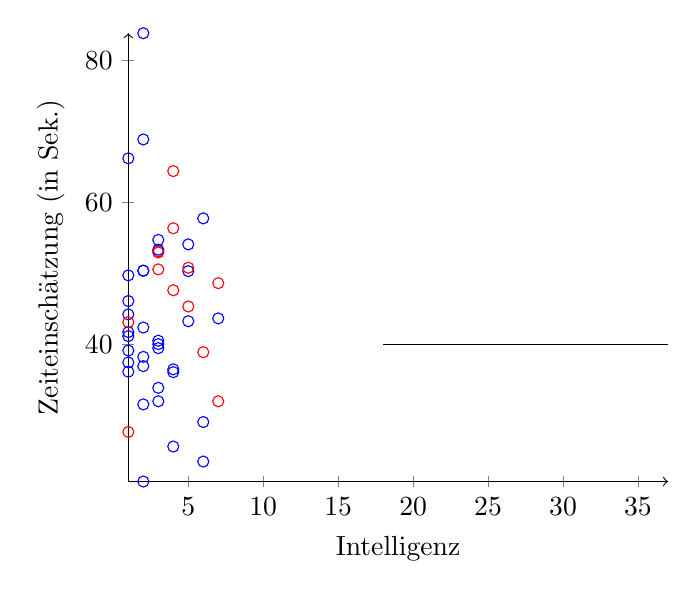
\begin{tikzpicture}
\begin{axis}[%
scatter/classes={%
    a={mark=o,draw=blue},
    b={mark=o,draw=red}},
    axis lines=middle,
    axis line style={->},
    x label style={at={(axis description cs:0.5,-0.1)},anchor=north},
    y label style={at={(axis description cs:-0.1,.5)},rotate=90,anchor=south},
    xlabel={Intelligenz},
    ylabel={Zeiteinschätzung (in Sek.)}]
  \addplot[domain=18:37]{40};
    \addplot[scatter,only marks,%
    scatter src=explicit symbolic]%
table[meta=label] {
x y label
1 46.08 a
1 27.6 b
1 44.19 a
1 39.1 a
1 41.13 a
1 37.42 a
1 41.7 a
1 43.1 b
1 66.23 a
1 49.7 a
1 36.1 a
2 42.34 a
2 31.49 a
2 50.36 a
2 50.36 a
2 38.2 a
2 83.89 a
2 36.89 a
2 20.6 a
2 68.89 a
3 50.55 b
3 40.00 a
3 53.1 b
3 33.83 a
3 53.33 a
3 40.48 a
3 52.94 b
3 54.71 a
3 31.93 a
3 39.43 a
4 36.04 a
4 56.35 b
4 47.6 b
4 25.54 a
4 64.42 b
4 36.44 a
5 50.3 a
5 54.08 a
5 45.31 b
5 50.78 b
5 43.23 a
6 29.00 a
6 57.75 a
6 23.42 a
6 38.86 b
7 48.6 b
7 43.63 a
7 31.93 b
	};
\end{axis}
\end{tikzpicture}
\caption{Zeiteinschätzung von 40 Sekunden mit Gespräch nach Müdigkeit}
\label{Zeit40sekGesprMued}
\end{minipage}
\hfill
\begin{filecontents}{data.csv}
dist
 46.08
 27.6 
 44.19 
 39.1 
 41.13 
 37.42 
 41.7 
 43.1 
 66.23 
 49.7 
 36.1 
 42.34 
 31.49 
 50.36 
 50.36 
 38.2 
 83.89 
 36.89 
 20.6 
 68.89 
 50.55 
 40.00 
 53.1 
 33.83 
 53.33 
 40.48 
 52.94 
 54.71 
 31.93 
 39.43 
 36.04 
 56.35 
 47.6 
 25.54 
 64.42 
 36.44 
 50.3 
 54.08 
 45.31 
 50.78 
 43.23 
 29.00 
 57.75 
 23.42 
 38.86 
 48.6 
 43.63 
 31.93  
\end{filecontents}
\begin{minipage}[t]{0.49\linewidth}
\begin{tikzpicture}
\begin{axis}[
    ybar,
    ymin=0
]
\addplot +[
    hist={
        bins=10,
        data min=0.5,
        data max=50
    }   
] table [y index=0] {data.csv};
\end{axis}
\end{tikzpicture}
\caption{Anzahl der Personen(y), welche die jeweilige Zeiteinschätzung(x) angaben - 40 Sekunden mit Gespräch nach Müdigkeit.}
\label{HistZeit40sekMitGesprMued}
\end{minipage}
\end{figure}


Auffällig ist hier, dass die stärksten Abweichungen gerade bei den Personen liegen, die am wenigsten müde sind.

\subsection{Zeitschätzungen}
\begin{figure}[H]
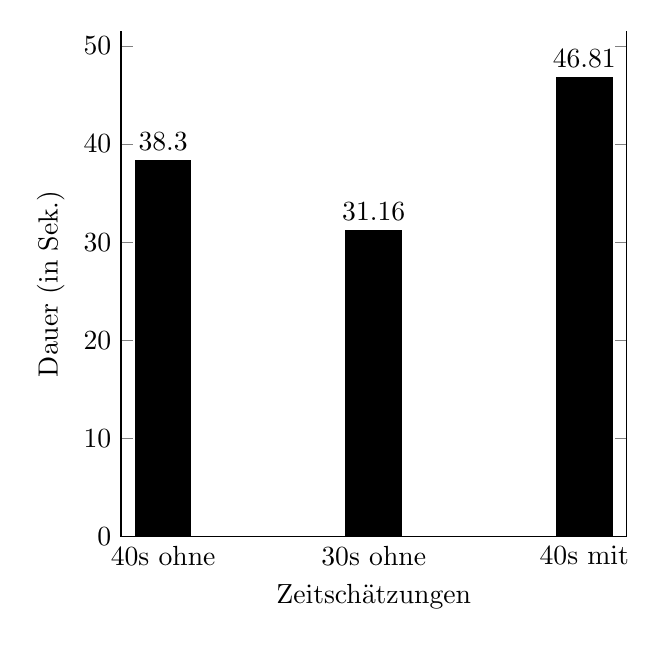
\begin{tikzpicture}
\begin{axis}[
     width  = 8cm,
     %hide y axis,
     axis x line*=bottom,
     height = 8cm,
     bar width=20pt,
     xlabel={Zeitschätzungen},
     ylabel={Dauer (in Sek.)},
     symbolic x coords={40s ohne,30s ohne,40s mit},
     nodes near coords,
     ymin=0,
     xtick=data
     ]
     
     \addplot[ybar, fill=black] coordinates {
          (40s ohne,38.30)
          (30s ohne,31.16)
          (40s mit,46.81)
          
     };
\end{axis}
\end{tikzpicture}
\caption{Gesamtheit aller Zeitschätzungen mit und ohne Gespräch}
\label{ZeitGespr}
\end{figure}
\par
Von links nach rechts sind dargestellt: die Einschätzungen von 40 Sekunden, dann 30 Sekunden und 40 Sekunden mit Gespräch als mögliche Beeinflussung. Auffällig ist, dass die dreißig Sekunden ziemlich genau getroffen wurden. Die Differenz zum Zielwert beträgt nicht einmal eine ganze Sekunde. Die vierzig Sekunden ohne das Gespräch, wurden durchschnittlich von den Versuchspersonen mit 36,41 um ca. vier Sekunden kürzer wahrgenommen. Die Variante mit dem Gespräch weist mit ca. 5 Sekunden Überschätzung der Zeit wie erwartet die größte Abweichung zum Zielwert auf, auch wenn sich dieser Differenzwert nicht sonderlich stark von dem des ersten Balken unterscheidet. Im Folgenden werden diese Werte separiert und als Versionen der Schätzungen vor und nach der VR dargelegt, um gegebenenfalls Einflüsse der VR ausfindig zu machen.
%%%%%%%%%%%%%%%%%%%%%%%%%%%%%%%%%%%%%%%%%%%%%%% vor der VR %%%%%%%%%%%%%%%%%%%%%%%%%%%%%%%
\begin{figure}[H]
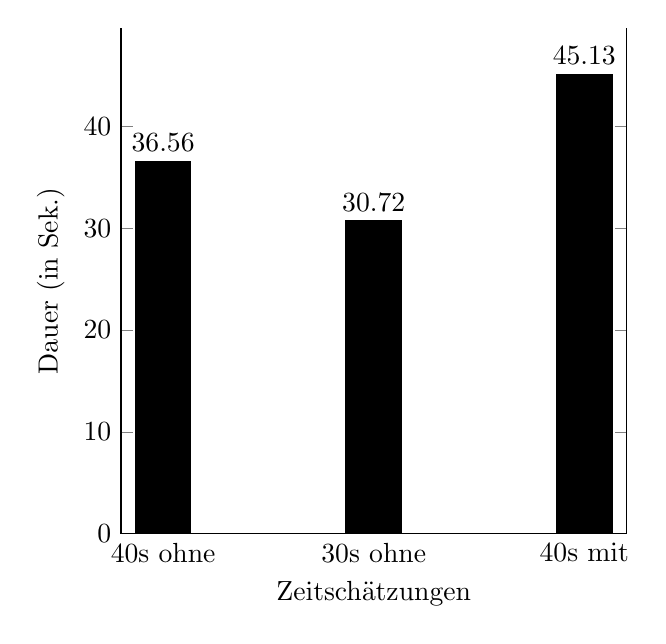
\begin{tikzpicture}
\begin{axis}[
     width  = 8cm,
     %hide y axis,
     axis x line*=bottom,
     height = 8cm,
     bar width=20pt,
     xlabel={Zeitschätzungen},
     ylabel={Dauer (in Sek.)},
     symbolic x coords={40s ohne,30s ohne,40s mit},
     nodes near coords,
     ymin=0,
     xtick=data
     ]
     
     \addplot[ybar, fill=black] coordinates {
          (40s ohne,36.56)
          (30s ohne,30.72)
          (40s mit,45.13)
          
     };
\end{axis}
\end{tikzpicture}
\caption{Zeitschätzung mit und ohne Gespräch vor der VR}
\label{ZeitVorVR}
\end{figure}

Hier sind die Zeit-Einschätzungen vor der VR dargestellt.
Die Schätzung der 30 Sekunden wird mit 30,72 Sekunden am präzisesten getroffen und die Zeitspanne der 40 Sekunden ohne Gespräch wird um ca. 3 Sekunden unterschätzt. Wieder schneidet die Schätzung mit dem Gespräch am schlechtesten ab. Die 40 Sekunden wurden um ca. 5 Sekunden länger geschätzt. 
 

%%%%%%%%%%%%%%%%%%%%%%%%%%%%%%%%%%%%%%%%%%%%%%%%% nach der VR %%%%%%%%%%%%%%%%%%%%%%%%%%%%%%%
\begin{figure}[H]
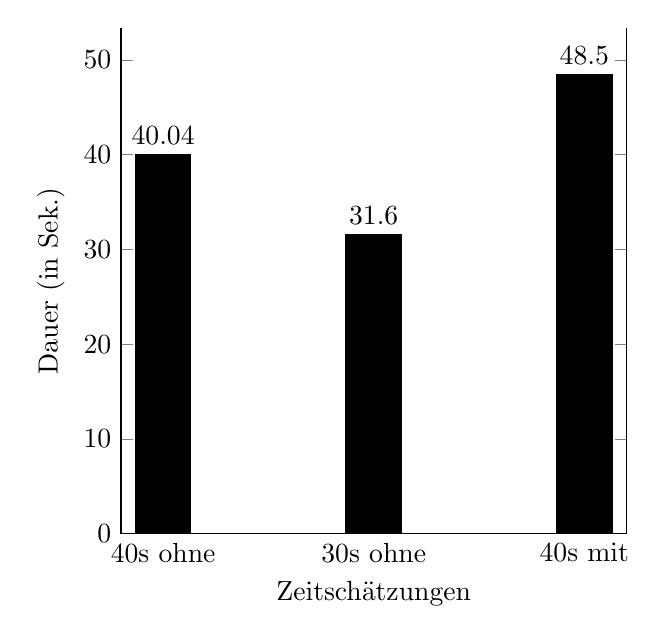
\begin{tikzpicture}
\begin{axis}[
     width  = 8cm,
     %hide y axis,
     axis x line*=bottom,
     height = 8cm,
     bar width=20pt,
     xlabel={Zeitschätzungen},
     ylabel={Dauer (in Sek.)},
     symbolic x coords={40s ohne,30s ohne,40s mit},
     nodes near coords,
     ymin=0,
     xtick=data
     ]
     
     \addplot[ybar, fill=black] coordinates {
          (40s ohne,40.04)
          (30s ohne,31.60)
          (40s mit,48.50)
          
     };
\end{axis}
\end{tikzpicture}
\caption{Zeitschätzung mit und ohne Gespräch nach der VR}
\label{ZeitNachVR}
\end{figure}

Hier abgebildet sind die jeweiligen Zeit-Einschätzungen nach der VR. 
Die 40 Sekunden ohne das Gespräch werden mit durchschnittlichen 40,04 Sekunden am genauesten getroffen. Darauffolgend die 31,06 Sekunden, der 30 Sekunden Abschätzung und am schlechtesten schneidet wieder die 40 Sekunden Schätzung mit dem Gespräch ab. Hier wird die Zeit um 8,5 Sekunden überschätzt.

%%%%%%%%%%%%%%%%%%%%%%%%%%%%%%%%%%%%%%%%%%%%%%%%%%%%%

\subsection{Einschätzung der vier Szenarien}
\newpage
Die tatsächliche Dauer aller Szenarien betrug achtzehn Sekunden. Die sich hier unterhalb befindliche Tabelle veranschaulicht je Szenario knapp den darin dargestellten Inhalt, die Art des Zeitgebers und unsere Erwartungen, ob die Zeitwahrnehmung dadurch entsprechend gedehnt oder verkürzt wird.
\begin{table}[H]
\centering
\begin{tabular}{llll}
	\hline
	\textbf{Szenario} & \textbf{Inhalt} & \textbf{Zeitgeber}& \textbf{Erwartungen} \\
	\hline
	a & LKW & a: schnelles Ticken & kürzer \\
	b & Vogel, Menschen & a: langsames Ticken & länger\\
	c & Park, Kind (rosa) & v: schnelles Schaukeln & kürzer\\
	d & Plakat, Kind (grün) & v: langsames Schaukeln & länger \\
	\hline
\end{tabular}
\caption{a=akustisch, v=visuell}
\label{AkVis}
\end{table}

Im Folgenden sind unsere tatsächlichen Ergebnisse des Experiments dargestellt: 

\begin{figure}[H]
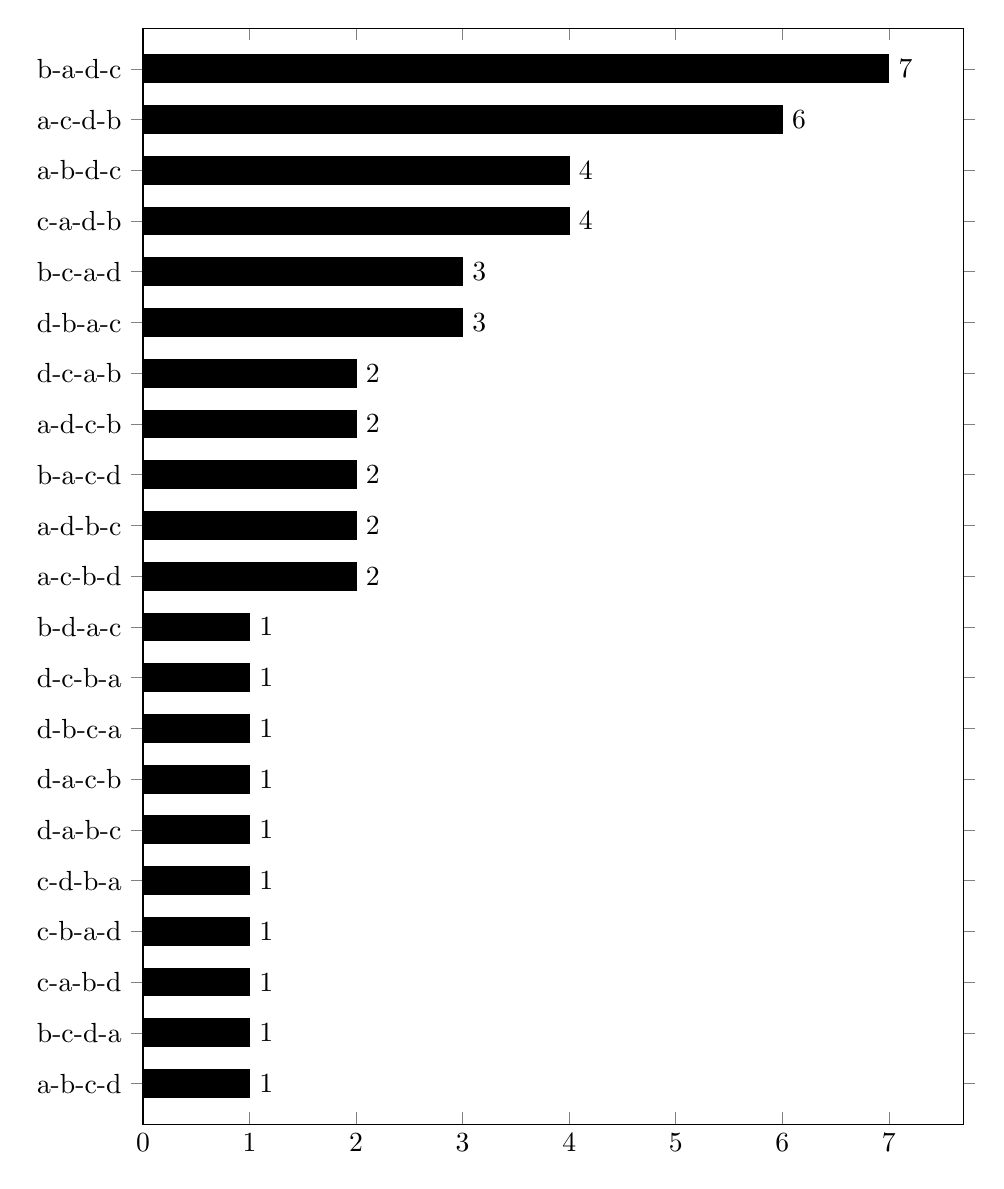
\begin{tikzpicture} 
\begin{axis}[ xbar, xmin=0, width=12cm, height=15.5cm, enlarge y limits=0.04, 
%xlabel={Probanden}, 
symbolic y coords={a-b-c-d,b-c-d-a,c-a-b-d,c-b-a-d,c-d-b-a,d-a-b-c,d-a-c-b,d-b-c-a,d-c-b-a,b-d-a-c,a-c-b-d,a-d-b-c,b-a-c-d,a-d-c-b,d-c-a-b,d-b-a-c,b-c-a-d,c-a-d-b,a-b-d-c,a-c-d-b,b-a-d-c}, 
ytick=data,
 nodes near coords,
  nodes near coords align={horizontal}, ] 
  
  
\addplot[xbar, fill=black] coordinates {
(1,a-b-c-d)
(1,b-c-d-a)
(1,c-a-b-d)
(1,c-b-a-d)
(1,c-d-b-a)
(1,d-a-b-c)
(1,d-a-c-b)
(1,d-b-c-a)
(1,d-c-b-a)
(1,b-d-a-c)
(2,a-d-c-b)
(2,a-c-b-d)
(2,a-d-b-c)
(2,b-a-c-d)
(2,d-c-a-b)
(3,d-b-a-c)
(3,b-c-a-d)
(4,c-a-d-b)
(4,a-b-d-c)
(6,a-c-d-b)
(7,b-a-d-c)
};
 \end{axis}
  \end{tikzpicture}
  \caption{Szenarien von kurz nach lang}
  \label{SzenarienKurzLang}
  \end{figure}

Oben zu sehen: die Anzahl der Probanden, die die Szenarien entsprechend von kurz nach lang sortiert haben. D.h. konkret, dass insgesamt sieben Probanden   \textbf{b} für das kürzeste Szenario hielten und dann aufsteigend über \textbf{a} und \textbf{d} nach  \textbf{c} sortiert haben. \\
Sechs Probanden waren der Ansicht, \textbf{a} sei das kürzeste Szenario gewesen, gefolgt von \textbf{c}, \textbf{d} und schließlich \textbf{b}.\\
Die geschätzte Länge der Szenarien kann man nach visuellen und akustischen Zeitgebern trennen:

	
\begin{figure}[H]
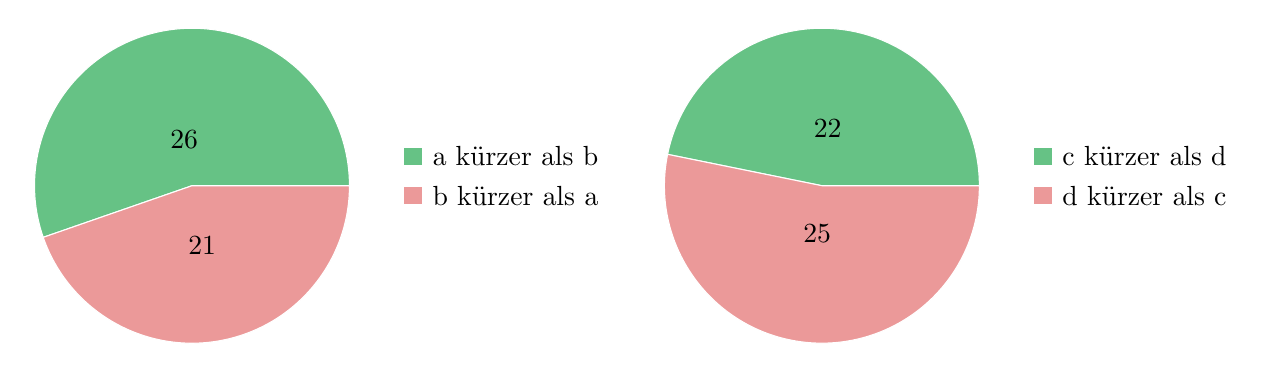
\begin{tikzpicture}
\tikzset{lines/.style={draw=white},}
\pie[color={greenOfApproval!60, redOfDisapproval!40},radius = 2 ,sum=auto, after number=,text=legend,every only number node/.style={text=black},style={lines}]{26/a kürzer als b,21/b kürzer als a}
\tikzset{lines/.style={draw=white},}
\pie[pos={8,0},radius = 2, color={greenOfApproval!60, redOfDisapproval!40},sum=auto, after number=,text=legend,every only number node/.style={text=black},style={lines}]{22/c kürzer als d,25/d kürzer als c}
\end{tikzpicture}
\caption{Links: Länge der akustischen Szenarien. Rechts: Länge der visuellen Szenarien}
\label{SzenarienVisuellAkustisch}
\end{figure} %[H]
	
	Die Tortendiagramme aus Abbildung 15 zeigen die beiden akustischen Szenarien \textbf{a} und \textbf{b} (links) und die visuellen Szenarien \textbf{c} und \textbf{d} jeweils in Relation zueinander. Hier sei nochmal erwähnt, dass jeweils die Szenarien \textbf{a} und \textbf{c} die kürzeren waren.\\
Durch die akustischen Zeitgeber haben 26 Probanden das Szenario \textbf{a} kürzer eingeschätzt als Szenario \textbf{b}. 21 Probanden waren gegenteiliger Meinung. Bei den visuellen Zeitgebern gibt es eine weniger eindeutige Meinung und das tatsächlich kürzere Szenario \textbf{c} haben 22 Personen erkannt, 25 schätzten \textbf{d} als kürzer ein.
	
	
Aus diesen Daten kann man herleiten, wie viele Personen ein Szenario als das kürzeste (Diagramm in gelb) bzw. längste (Diagramm in lila) empfunden haben. 

\begin{figure}[ht]
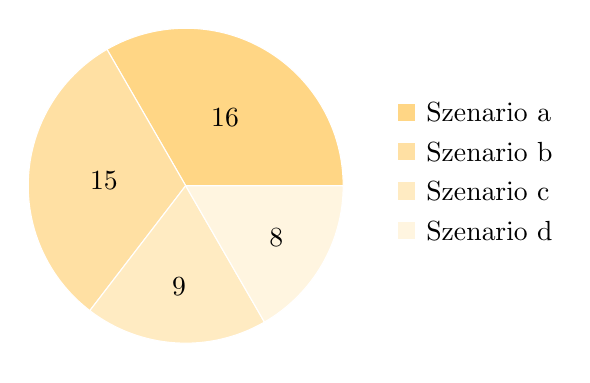
\begin{tikzpicture}
\tikzset{lines/.style={draw=white},}
\pie[color={yellowOfBrevity!80, yellowOfBrevity!60, yellowOfBrevity!40, yellowOfBrevity!20},radius = 2 ,sum=auto, after number=,text=legend,every only number node/.style={text=black},style={lines}]{16/Szenario a,15/Szenario b,9/Szenario c, 8/Szenario d}
\end{tikzpicture}
\caption{Welches Szenario war das kürzeste?}
\label{SzenarienKurz}
\end{figure}
	
Von allen Probanden haben 15 angegeben Szenario \textbf{a} als das kürzeste empfunden zu haben, knapp dahinter steht Szenario \textbf{b} mit 14 Stimmen. Im Vergleich dazu sind die Szenarien \textbf{c} und \textbf{d} mit 9 und 8 Stimmen etwas abgeschlagen. Eine eindeutige Mehrheit gibt es dennoch nicht.\\
Gleichermaßen kann man feststellen, welches Szenario von den meisten Personen als das längste bewertet wurde:

\begin{figure}[ht]
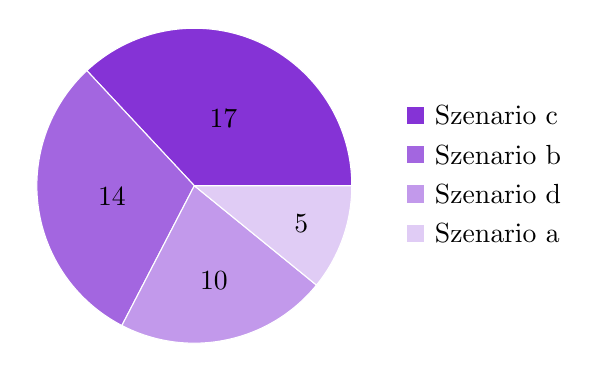
\begin{tikzpicture}
\tikzset{lines/.style={draw=white},}
\pie[color={purpleOfLengthiness!80, purpleOfLengthiness!60, purpleOfLengthiness!40, purpleOfLengthiness!20},radius = 2 ,sum=auto, after number=,text=legend,every only number node/.style={text=black},style={lines}]{17/Szenario c,14/Szenario b,10/Szenario d, 5/Szenario a}
\end{tikzpicture}
\caption{Welches Szenario war das längste?}
\label{SzenarienLang}
\end{figure}	

Auch bei der Bewertung des \textit{längsten} Szenarios gibt es keine ganz klare Mehrheit, dennoch heben sich zwei Szenarien etwas ab. 17 Versuchspersonen sind der Meinung, Szenario \textbf{c} sei das längste gewesen, danach kommen die Szenarien \textbf{b} mit 14 Stimmen und \textbf{d} mit 10 Stimmen. Abgeschlagen zum Schluss wird Szenario \textbf{a} mit nur 5 Stimmen genannt.\\
Auffällig ist, dass es keine einheitliche Meinung gibt, welches Szenario das längste oder kürzeste ist, allerdings zeichnen sich ein paar Tendenzen ab. So ist sich die relative Mehrheit der Versuchspersonen sicher, \textbf{a} sei das längste Szenario und dementsprechend wenige behaupten das direkte Gegenteil. Ähnlich verhält es sich bei Szenario \textbf{c}, welches auch verhältnismäßig oft als das längste bewertet wurde und nur sehr wenig als das kürzeste.\\
Auffällig ist allerdings auch, dass die Meinungen bei \textbf{b} recht stark auseinandergehen. Ein Großteil der Befragten sieht dieses Szenario entweder als das längste oder als das kürzeste an, es gibt nur wenig Verteilung im Mittelbereich.
	
	
	
	%%%%%%%%%% DURCHSCHNITTZEITEN DER SZENARIEN
\begin{figure}	[H]
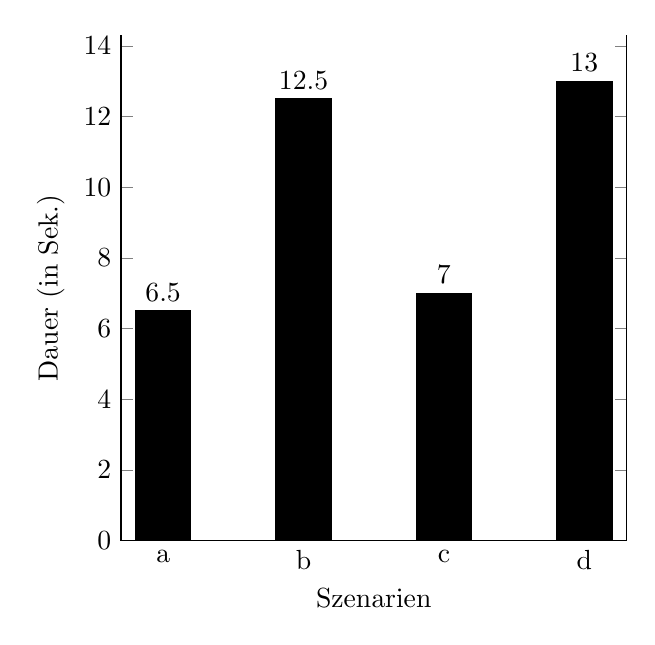
\begin{tikzpicture}
\begin{axis}[
     width  = 8cm,
     %hide y axis,
     axis x line*=bottom,
     height = 8cm,
     bar width=20pt,
     symbolic x coords={a,b,c,d},
     xlabel={Szenarien},
     ylabel={Dauer (in Sek.)},
     nodes near coords,
     ymin=0,
     xtick=data
     ]
     
     \addplot[ybar, fill=black] coordinates {
          (a,6.5)
          (b,12.5)
          (c,7)
          (d,13)
     };
\end{axis}
\end{tikzpicture}
\caption{Durchschnittlich geschätzte Längen der Szenarien}
\label{LaengeSzenarien}
\end{figure}
\par
Die zeitlichen Einschätzungen bezüglich der Längen der einzelnen Szenarien sind als ermittelte Durchschnittswerte im obigen Balkendiagramm je Szenario dargestellt. Hier zu erkennen ist nun, dass das Szenario \textbf{d} mit durchschnittlichen 13 Sekunden als das Längste eingeschätzt wurde. Knapp dahinter liegt \textbf{b} mit 12,5 Sekunden, gefolgt von \textbf{a} mit 6,5 und \textbf{c} mit 7 Sekunden durchschnittlicher Schätzung.
%Interessant ist, dass eine Differenz von 0,5 Sekunden sowohl zwischen \textbf{a} und \textbf{c}, als auch \textbf{b} und \textbf{d} zu finden ist. Außerdem werden \textbf{b} und \textbf{d} nahezu doppelt solang geschätzt wie \textbf{a} und \textbf{c}.

\subsection{Beziehung zwischen Spaß- und Zeitempfinden}
\par
Ein Faktor der die Zeitwahrnehmung beeinflusst haben könnte, ist hinsichtlich des Forschungspapiers "'Kinder, wie die Zeit vergeht!"'
\textit{Über Paradoxien in der Zeitwahrnehmung von Katja Irle} \cite{Irle2017} der Spaß am Geschehen.
Hierzu unsere Ergebnisse:
	
\begin{figure}[H]
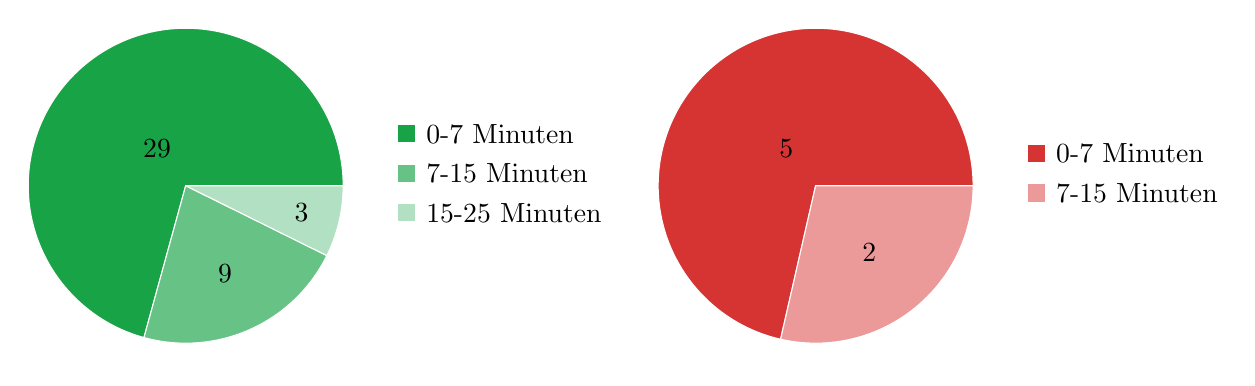
\begin{tikzpicture}
\tikzset{lines/.style={draw=white},}
\pie[color={greenOfApproval!90, greenOfApproval!60, greenOfApproval!30},radius = 2 ,sum=auto, after number=,text=legend,every only number node/.style={text=black},style={lines}]{29/0-7 Minuten,9/7-15 Minuten,3/15-25 Minuten}


\tikzset{lines/.style={draw=white},}
\pie[pos={8,0},radius = 2, color={redOfDisapproval!80, redOfDisapproval!40},sum=auto, after number=,text=legend,every only number node/.style={text=black},style={lines}]{5/0-7 Minuten,2/7-15 Minuten}
\end{tikzpicture}
\caption{Links: Spaß. Rechts: \textit{kein} Spaß}
\label{Spass}
\end{figure} %[H]

Die obigen beiden Tortendiagramme stellen unsere Versuchspersonen separiert dar. Links die Gruppe derer die Spaß an ihrem VR-Aufenthalt hatten und rechts die Versuchspersonen die angaben, dass sie keinen Spaß hatten. Innerhalb dieser Gruppen sind die Zeitschätzungen des VR-Aufenthalts abgebildet.Von den 41 Versuchspersonen die Spaß hatten, hat eine klare Mehrheit von 29 Personen geschätzt, dass die Dauer ihres VR-Aufenthalts im Intervall von 0-7 Minuten liegt. Weitere 9 Personen wählten die Zeitspanne von 7-15 Minuten und lediglich 3 schätzten die Dauer länger als 15 Minuten. Im rechten Tortendiagramm sind 7 Personen abgebildet, davon hat wieder die Mehrheit geschätzt, dass sie bis zu 7 Minuten in der VR waren und die restlichen 2 wählten das Intervall von 7-15 Minuten. Insgesamt entschieden sich also ca. 70\% von den insgesamt 48 Versuchspersonen für eine Zeitspanne von bis zu 7 Minuten. Was sich durch die im Rahmen haltende Größe unserer Welt und der Geschwindigkeit mit der man sich darin bewegen kann, eigentlich auch hätte erahnen lassen können.

\par
Da die Intervalle zur Zeiteinschätzung des Aufenthalts in der VR von uns ungünstig gewählt wurden (Verbesserungsvorschläge hierzu, siehe in der Methodenkritik des Fazits), beziehen wir uns im Folgenden nur noch auf die tatsächliche Dauer, die von uns während der Versuchsdurchführung aufgenommen wurde. 

	\begin{figure}[H]
	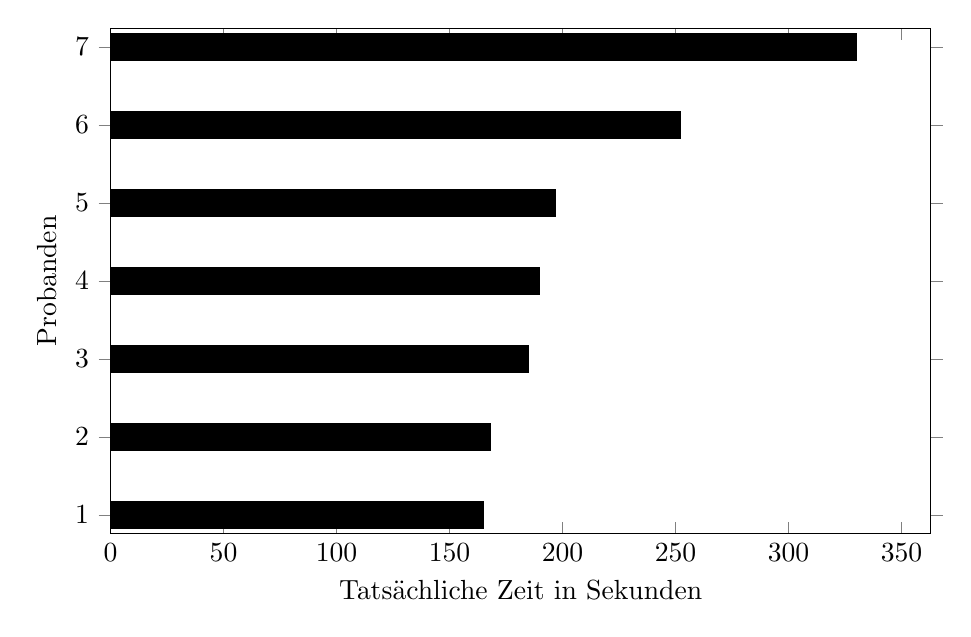
\begin{tikzpicture} 
\begin{axis}[ xbar, xmin=0, width=12cm, height=8cm, enlarge y limits=0.04, 
xlabel={Tatsächliche Zeit in Sekunden},ylabel={Probanden}, 
symbolic y coords={1,2,3,4,5,6,7}, 
ytick=data,
% nodes near coords,
 % nodes near coords align={horizontal}, 
 ] 
 
\addplot[xbar, fill=black] coordinates {
(165,1)
(168,2)
(185,3)
(190,4)
(197,5)
(252,6)
(330,7)
};
 \end{axis}
  \end{tikzpicture}
  \caption{Tatsächliche Zeit der Versuchspersonen, die keinen Spaß hatten}
  \label{ZeitKeinSpass}
  %DURCHSCHNITT: 212,42 sek
	\end{figure}
In diesem Balkendiagramm wird die von uns aufgenommene tatsächliche Dauer des VR-Aufenthalts der sieben Versuchspersonen dargestellt, die nach eigener Angabe keinen Spaß an der Durchführung hatten. Das Minimum beträgt hier 165 Sekunden, also 2,75 Minuten, das Maximum beträgt 330 Sekunden, das sind 5,50 Minuten und der Median entspricht 190 Sekunden, also 3,16 Minuten. Die ersten fünf Zeiten liegen verhältnismäßig nah beieinander. Die unteren beiden Balken betrachtend, hielten sich die betreffenden Versuchspersonen länger in der VR auf.


		\begin{figure}[H]
	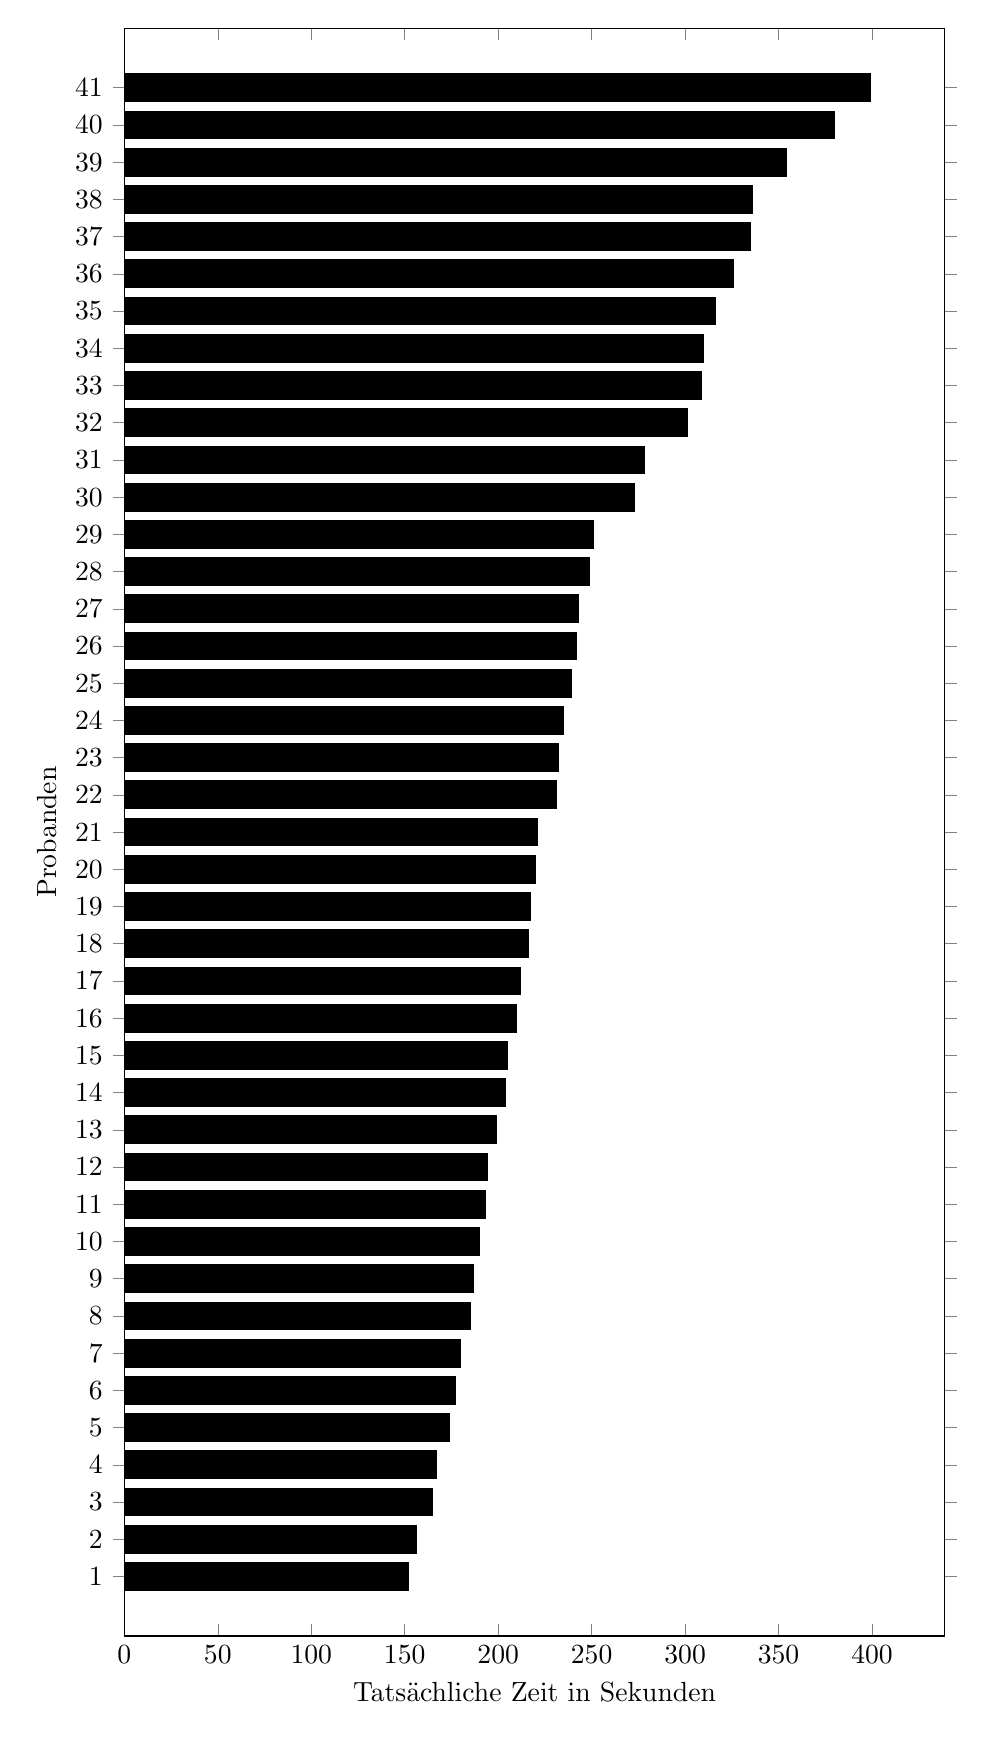
\begin{tikzpicture} 
\begin{axis}[ xbar, xmin=0, width=12cm, height=22cm, enlarge y limits=0.04, 
xlabel={Tatsächliche Zeit in Sekunden},
ylabel={Probanden}, 
symbolic y coords={1,2,3,4,5,6,7,8,9,10,11,12,13,14,15,16,17,18,19,20,21,22,23,24,25,26,27,28,29,30,31,32,33,34,35,36,37,38,39,40,41},
ytick=data,
% nodes near coords,
 % nodes near coords align={horizontal}, 
 ] 
 
\addplot[xbar, fill=black] coordinates {
(152,1)
(156,2)
(165,3)
(167,4)
(174,5)
(177,6)
(180,7)
(185,8)
(187,9)
(190,10)
(193,11)
(194,12)
(199,13)
(204,14)
(205,15)
(210,16)
(212,17)
(216,18)
(217,19)
(220,20)
(221,21)
(231,22)
(232,23)
(235,24)
(239,25)
(242,26)
(243,27)
(249,28)
(251,29)
(273,30)
(278,31)
(301,32)
(309,33)
(310,34)
(316,35)
(326,36)
(335,37)
(336,38)
(354,39)
(380,40)
(399,41)
};
 \end{axis}
  \end{tikzpicture}
  \caption{Tatsächliche Zeit der Versuchspersonen, die Spaß hatten}
  \label{ZeitSpass}
  %DURCHSCHNITT: 240,56s
	\end{figure}
	Analog zum vorherigen Balkendiagramm werden hier auch die tatsächlichen Zeiten der VR-Aufenthalte veranschaulicht, nur mit dem Unterschied, dass es sich hier um jene Personen handelt die nach eigenen Angaben Spaß am Geschehen empfunden hatten.
Die Wertespanne beginnt unten mit einem Minimum von 152 Sekunden, umgerechnet sind das ca. 2,5 Minuten und endet oben mit dem Maximum von 399 Sekunden oder auch als Minutenwert, 6,65. Der Median liegt bei 221 Sekunden, also 3,68 Minuten. Die ersten größeren zeitlichen Sprünge lassen sich im Bereich der oberen zwölf Versuchspersonen beobachten, insbesondere hinsichtlich der ersten beiden. Der Wertebereich $[165-330]$ aus dem vorherigem Diagramm ist auch in das hier Betrachtete inkludiert. Somit sind abgesehen davon, dass es sich hier um weitaus mehr Beteiligte handelt, keine sonderlichen Verschiedenheiten zwischen den beiden Varianten bemerkbar.
	
\newpage

\subsection{Bewertung der Szenarien}
	\begin{figure}[ht]
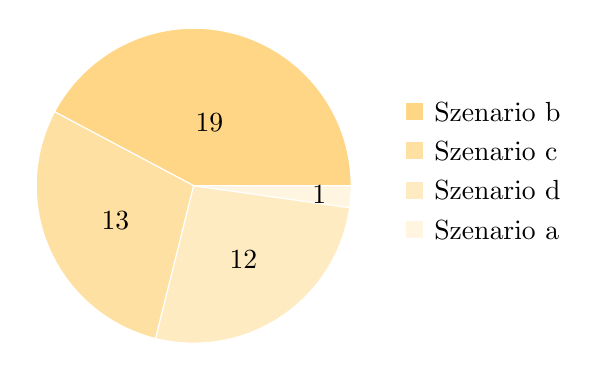
\begin{tikzpicture}
\tikzset{lines/.style={draw=white},}
\pie[color={yellowOfBrevity!80, yellowOfBrevity!60, yellowOfBrevity!40, yellowOfBrevity!20},radius = 2 ,sum=auto, after number=,text=legend,every only number node/.style={text=black},style={lines}]{19/Szenario b,13/Szenario c,12/Szenario d, 1/Szenario a}
\end{tikzpicture}
\caption{Welches war das beste Szenario?}
\label{SzenarioGut}
\end{figure}

Die Mehrheit der Versuchspersonen stimmt mit 19 Stimmen für Szenario \textbf{b} als das beste. \textbf{c} und darauffolgend \textbf{d} liegen im Mittelfeld. Weit abgeschlagen mit nur einer Stimme steht Szenario \textbf{a} auf dem letzten Platz.
	
	
	\begin{figure}[ht]
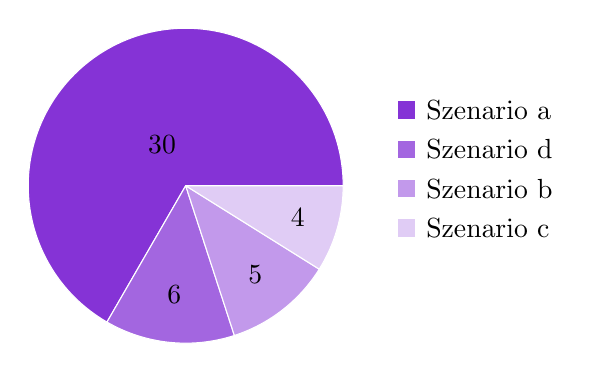
\begin{tikzpicture}
\tikzset{lines/.style={draw=white},}
\pie[color={purpleOfLengthiness!80, purpleOfLengthiness!60, purpleOfLengthiness!40, purpleOfLengthiness!20},radius = 2 ,sum=auto, after number=,text=legend,every only number node/.style={text=black},style={lines}]{30/Szenario a,6/Szenario d,5/Szenario b, 4/Szenario c}
\end{tikzpicture}
\caption{Welches war das schlechteste Szenario?}
\label{SzenarioSchlecht}
\end{figure}
	

Bei der Frage nach dem schlechtesten Szenario sind sich ca. 67\% Prozent der Versuchspersonen einig, dass ihnen \textbf{a} am wenigsten gefallen hat. Deutlich abgeschlagen mit nur 6, 5 und 4 Stimmen die Szenarien \textbf{d}, \textbf{b} und \textbf{c}. 
Bei der Sortierung von \textit{gut} nach \textit{schlecht} fällt auf, dass gerade Szenario \textbf{a} wieder eine klare Tendenz hat und es als allgemein schlechter wahrgenommen wurde als alle anderen.


\section{Diskussion}

\subsection{Scatterplots: Einflüsse auf die Zeitwahrnehmung}
Zu Beginn der Auswertung wurde versucht, Variablenpaare unserer gesammelten Werte in Beziehung zueinander zu setzen und dafür Scatterplots zu erstellen. Zuvor erfolgte bereits eine Auseinandersetzung damit, welche Faktoren die Zeitwahrnehmung beeinflussen können: so kann sie z.B. mit jungem/höherem Alter, mit einer tiefen/hohen Körpertemperatur, einer niedrigen/ hohen Intelligenz, bei Müdigkeit sowie unter den Geschlechtern variieren. Herausgestellt wurden diese Beeinflusser von Pascal Wallisch in seinem Paper "'Zeiterleben in der Tempogesellschaft"' \cite{Wallisch2003}. Ob diese Faktoren auch unsere Versuchspersonen beeinflusst haben, soll herausgestellt werden.

\paragraph{Zu Abb. \ref{Zeit40sek}-\ref{HistZeit30sek}:}
Zunächst wird überprüft, ob das Alter auch in unserem Experiment Einfluss auf die Zeitwahrnehmung hatte, jedoch ergeben die Werte der geschätzten Zeiten von 40 und 30 Sekunden (jeweils ohne Ablenkung) kein eindeutiges Bild. Auch wenn die Ausreißer im Diagramm unbeachtet bleiben, ist keine Abhängigkeit zwischen den Variablen "'Zeiteinschätzung"' und "'Alter"' zu erkennen. Zusätzlich bleibt die Verteilung von Männern und Frauen unauffällig. Ein Grund dafür kann sein, dass die Anzahl der Teilnehmer mit einem Alter über 30 Jahren nicht groß genug gewesen ist oder generell eine größere Probandenanzahl erforderlich gewesen wäre.

\paragraph{Zu Abb. \ref{Zeit40sekInt}-\ref{HistZeit30sekInt}:} Auch die Variablen "'Intelligenz"' und "'Zeiteinschätzung"' bleiben ohne bei der 30- und der 40-Sekunden-Einschätzung sichtbare Beziehung, der Männer- und Frauenanteil scheint gleichmäßig verteilt. So kann zum Bespiel nicht daraus geschlossen werden, dass eine höhere Intelligenz auch mit einem besseren Zeiteinschätzungsvermögen verbunden ist. Dies könnte unter anderem damit zusammenhängen, dass lediglich eine Kurzform eines Intelligenztests verwendet wurde, der zudem stark mit den sprachlichen Fähigkeiten der jeweiligen Versuchsperson zusammenhing (vor allem für Nicht-Muttersprachler eine Schwierigkeit). Es wäre möglich, die Intelligenz vor dem Experiment noch exakter zu überprüfen. Zudem hätte eine größere Probandengruppe wiederum zu einem genaueren Ergebnis führen können.

\paragraph{Zu Abb. \ref{Zeit40sekTemp}-\ref{HistZeit30sekTemp}:} Ebenfalls bei beiden Einschätzungen keine Beziehung erkennen lässt sich zwischen den Variablen "'Temperatur"' und "'Zeiteinschätzung"', auffällig sind hier allenfalls einige Ausreißer, die sich durch ein sehr schlechtes Zeiteinschätzungsvermögen und/oder Messfehler erklären lassen. Männer und Frauen sind abermals gleichmäßig verteilt. Auch hier hätte vielleicht eine größere Probandengruppe zu einem differenzierteren Ergebnis führen können.

\paragraph{Zu Abb. \ref{Zeit40sekMued}-\ref{HistZeit30sekMued}:} Sehr gleichmäßig verteilt zeigen sich der Werte des Variablenpaar "'Zeiteinschätzung"' und "'Müdigkeit"' bei der 30- und der 40-Sekunden-Schätzung, worunter auch die Verteilung des Männer- und Frauenanteils keine Auffälligkeiten zeigt. Jedoch haben dabei insgesamt nur wenige Versuchspersonen teilgenommen, die sich selbst als sehr müde einschätzten - wieder könnte ein größere Anzahl das Ergebnis verändern. Zudem erfolgte die Einteilung der Müdigkeitsstufen nach Selbsteinschätzung, die keine vollkommene Zuverlässigkeit erreichen kann. 

\paragraph{Zu Abb. \ref{Zeit40sekAltMitGespr}-\ref{HistZeit40sekMitGesprMued}:} Die abschließenden Scatterplots und Histogramme untersuchen, ob sich die Zeiteinschätzung unter Einfluss der einzelnen Faktoren Geschlecht, Intelligenz, Alter, Temperatur und Müdigkeit verändert, wenn die Versuchspersonen während der Zeitschätzung durch ein Gespräch abgelenkt werden. Jedoch ist auch bei einer Ablenkung keine Beziehung zwischen der "'Zeiteinschätzung"' und der jeweiligen anderen Variable zu erkennen; die Ablenkung scheint in dieser Hinsicht keinen Einfluss genommen zu haben.\\ 

Eindeutige Ergebnisse lassen sich somit aus den einzelnen Scatterplots nicht ablesen. So ist z.B. auf keinem Diagramm eine lineare Abhängigkeit zu erkennen, sodass das Berechnen einer Korrelation erfolgen könnte. Dieses Resultat bedeutet jedoch nicht, dass die genannten Faktoren keinen Einfluss auf unsere Versuchspersonen hatten, nur ist der Einfluss nicht aus den Werten ablesbar. Bereits genannte Gründe dafür könnte unter anderem sein, dass unsere Probandenanzahl im Vergleich zu anderen Untersuchungen zu gering ausfiel, um genaue Ergebnisse zu erzielen. Auch kann es sich um ungenaue Messungen handeln, so wurde z.B. lediglich eine Kurzform eines Intelligenztests verwendet.

\subsection{Zeitschätzungen}
\paragraph{Zu Abb.\ref{ZeitGespr}:} Die Durschnittswerte der Zeitabschätzungen der Versuchspersonen zeigen, dass es ihnen tendenziell leichter fiel, kürzere Zeiten (30 Sekunden) zu schätzen als längere (40 Sekunden) -- das Diagramm zeigt, dass die Abweichung der Schätzungen hier um 0,7 Sekunden geringer ausfällt. Da sich alle Versuchspersonen für knapp 3 Minuten und länger in der VR-Welt aufhielten, ist davon auszugehen, dass eine Abschätzung dieser Zeit nochmals unzuverlässiger ausfallen wird, als die der 40 Sekunden. Zudem ist zu erkennen, dass Ablenkung das Ergebnis verschlechtert -- die Zeit wurde als deutlich länger geschätzt, sobald ein Gespräch geführt wurde. Da auch der VR-Aufenthalt auditive und zusätzlich visuelle Ablenkung bietet, kann vermutet werden, dass auch dieser länger, als real stattgefunden, eingeschätzt wird.\\
Eine Versuchsperson hielt sich durchschnittlich 237,8 Sekunden in der VR-Welt auf, diese Zeit sollte er nach dem Experiment selbst abschätzen. Hier wäre es interessant zu erfahren, ob das Zeitempfinden sich, wie vermutet, wirklich beschleunigt hat, jedoch verhindern zu groß gewählte Zeitspannen (die kleinste betrug 0-7 Minuten) ein eindeutiges Ergebnis. Auf das betreffende Diagramm \ref{Spass} wird später noch Bezug genommen.

\paragraph{Zu Abb. \ref{ZeitVorVR} und Abb. \ref{ZeitNachVR}:} Im Vergleich der beiden Diagramme ist zu erkennen, dass die Versuchspersonen die Zeit nach ihrem Aufenthalt in der VR-Welt stärker überschätzten als vor dem Aufenthalt. Während die 40 Sekunden ohne Ablenkung bei der zweiten Schätzung exakter ausfielen, entstand bei der Schätzung von 30 Sekunden ohne Ablenkung und der von 40 Sekunden mit Ablenkung eine Verschlechterung durch eine zu lange Einschätzung der Zeit. Noch stärker als bei der ersten Messung stellt sich heraus, dass eine Ablenkung durch ein Gespräch während der Zeitschätzung zu einem schlechteren Ergebnis bzw. zu einer Überschätzung der Zeit führt.

\subsection{Einschätzung der vier Szenarien}
\paragraph{Zu Abb. \ref{SzenarienKurzLang}-\ref{LaengeSzenarien}:} Abbildung \ref{SzenarienKurzLang} stellt die Anzahl dar, wie oft welche Szenarioreihenfolge gewählt wurde, allerdings lassen sich keine Rückschlüsse auf die zuvor festgelegten Hypothesen oder die am Anfang des Experiments von der Versuchsperson erfragten Variablen schließen. Aufgrund dessen werden die Szenarien wie in Abbildung \ref{SzenarienVisuellAkustisch}
nach den Faktoren visuell und akustisch getrennt. Nahezu die Hälfte aller Versuchspersonen haben die schnellen Szenarien wirklich als schneller wahrgenommen. Dabei ist auffällig, dass bei den akustischen Szenarien 55,3\% der Personen \textbf{a} tatsächlich als schneller eingestuft haben. Bei den visuellen Szenarien wurde das schnelle Szenario \textbf{c} allerdings nur zu 46,8\% erkannt. Daraus kann geschlussfolgert werden, dass es sich bei den akustischen Zeitgebern um die effektiveren handelt, die den Versuchspersonen im Vergleich zu den visuellen Szenarios erfolgreicher beeinflusst haben.

In den Kreisdiagrammen \ref{SzenarienKurz} und \ref{SzenarienLang} werden die Szenarien nach ihrer Länge sortiert: Ersteres stellt die Anzahl dar, wie oft die Szenarien jeweils als kürzestes wahrgenommen worden sind und das Zweite wie oft die Szenarien jeweils als längstes eingeschätzt worden sind. Allerdings besteht ein Zweifel der Richtigkeit der Daten. Wo Szenario \textbf{b} in der ersten Abbildung als zweit kürzestes dargestellt wird, ist es auch gleichzeitig das zweit längste Szenario in der zweiten Darstellungsform. Grund dafür sind möglicherweise die nicht korrekt ausgefüllten Fragebögen der Versuchspersonen. Einige trugen zwar die ihrer Meinung nach richtige Reihenfolge ein, allerdings erhielten einige Szenarien, die sich vor dem längsten befunden hatten, eine zum Teil längere Dauer, als das längste Szenario.\\ Aufgrund dessen lässt sich die Darstellungs \ref{SzenarienKurzLang} besser interpretieren, denn bei den ermittelten Durchschnittswerten der
geschätzten Längen der Szenarien lässt sich eine Besonderheit feststellen:
Es gibt ähnliche Schätzwerte bei Szenario \textbf{a} und \textbf{c}, sowie bei
\textbf{b} und \textbf{d}. In Szenario
\textbf{a} und \textbf{c} wurde die Versuchsperson durch einen schnelleren Zeitgeber
beeinflusst, in Szenario \textbf{b} und \textbf{d} durch einen langsameren.
Die eine Hypothese war es, dass das Zeitgefühl durch schnelle Zeitgeber so beeinflusst
wird, dass die Zeit für die Versuchspersonen gefühlt schneller vergeht. Anhand des
Diagramms lässt sich eindeutig erkennen, dass dies für die schnelleren Szenarien
zutrifft und der geschätzte Durchschnittswert jeweils deutlich unter der
tatsächlichen Länge von 18 Sekunden liegt. Das Ergebnis der langsamen Szenarien \textbf{b} und
\textbf{d} unterscheidet sich zwar stark von den Ergebnissen der schnellen
Szenarien und zeigt, dass diese eindeutig länger eingeschätzt wurden, allerdings
entsprechen sie nicht der zu Beginn festgelegten zweiten Hypothese: Die Zeit vergeht 
gefühlt langsamer, wenn eine Person durch einen langsamen Zeitgeber beeinflusst wird. Die
tatsächliche Länge von 18 Sekunden wurde somit deutlich verfehlt, allerdings zeigt es dennoch
die unterschiedliche Wirkungen von den schnellen und langsamen Zeitgebern, auch wenn es keinen
deutlichen Unterschied zwischen den beiden Arten der Zeitgeber gibt. Dies lässt sich vermutlich
darauf zurückführen, dass die Zeitintervalle der einzelnen Szenarien nicht direkt, während sich
die Versuchsperson in der VR-Welt befunden hatte, sondern erst im Nachhinein eingeschätzt werden mussten.
Somit wurde nicht nur die Fähigkeit, Zeit richtig einschätzen zu können, sondern
ebenfalls das Erinnerungsvermögen gefordert.

\subsection{Beziehung zwischen Spaß- und Zeitempfinden}
\paragraph{Zu Abb. \ref{Spass}-\ref{ZeitSpass}:} Nach dem Aufenthalt der Versuchsperson in der VR-Welt wurden diese nach ihrem Spaßempfinden befragt. Dieses Ergebnis kann damit erklärt werden, dass die bereits gewählten Zeitspannen letztendlich nicht mehr auf unser Experiment, das zwischenzeitlich noch stark verändert wurde, passten. Geschickter wären kleinere Zeitspannen (0-2 Minuten, 3-4 Minuten,...) gewesen.\\
Unsere Vermutung vor dem Experiment war es, dass die Zeit gefühlt schneller vergeht, wenn man gerade etwas Positives oder generell geistig Aktives erlebt. Zu diesem Schluss ist auch der Psychologe Helmut Prior gekommen: "'Momente, in denen wir extrem angespannt oder aufgeregt sind, bleiben eher in der Erinnerung und kommen uns hinterher tendenziell lang vor."' \cite{Irle2017} \\
Diese Hypothese lässt sich durch unsere Ergebnisse nicht belegen, da der Anteil der Versuchspersonen beider Gruppen, die die Dauer im korrekten Zeitfenster geschätzt haben, bei gerundeten 71 Prozent liegt. Dies ist ein weiterer Anhaltspunkt für die bereits erwähnten unpassend gewählten Zeitspannen.\\
Somit lassen sich keine Resultate aus den oben dargestellten Ergebnissen schließen.

\subsection{Bewertung der Szenarien}
\paragraph{Zu Abb. \ref{SzenarioGut}-\ref{SzenarioSchlecht}:} Aus dem Vergleich der beiden Diagramme, die die Probandenbefragung nach dem besten (Abb. \ref{SzenarioGut}) und schlechtesten Szenario (Abb. \ref{SzenarioSchlecht}) darstellen, geht Szenario "'a"' (Zeitgeber: schnelles Ticken) als eindeutig am schlechtesten bewertetes hervor. Es wurde bei der Wahl des besten Szenarios auf den letzten und bei der Wahl des schlechtesten Szenarios auf den ersten Platz gesetzt. Dagegen hebt sich das Szenario "'b"' (langsames Ticken) positiv hervor; es ist erstplatziert bei der Wahl des besten Szenarios und befindet sich bei der Wahl des schlechtesten auf dem vorletzten Platz. Dies ist gegenteilig wie erwartet, da zuvor vermutet wurde, dass schnelle Zeitgeber auch ein schnelleres Zeitempfinden erzeugen und dieses wiederum auch mit Spaßempfinden verbunden ist.\\
Der These nach, dass das beste Szenario -- das mit dem größten Spaßempfinden -- auch dem als am kürzesten empfunden entspricht, müsste die Reihenfolge der Abb. \ref{SzenarienKurzLang} (Sortierung der Szenarien von kurz nach lang) nun "'b c d a"' ergeben. Tatsächlich wurde "'a"' jedoch am häufigsten (17 von 47 Einschätzungen) an erster Stelle angegeben, "'b"' ist erst an zweiter Stelle zu finden (14 von 47 Einschätzungen).\\ 
Auch im Vergleich mit den Abb. \ref{SzenarienKurz} und \ref{SzenarienLang} konnte damit die These, dass bei Spaßempfinden die Zeit gefühlt schneller vergeht, in unserem Experiment nicht belegt werden. In den soeben genannten Diagrammen wurde das am schlechtesten empfundene Szenario "'a"' als eindeutig kürzestes festgelegt, was bedeutet, dass die kürzeste Zeitspanne in dem Fall am wenigsten Spaß hervorgerufen hat. Das Szenario "'b"' wurde in beiden Wahlen (schnellstes und langsamstes Szenario) an zweiter Stelle gewählt und lässt sich damit nicht sicher einordnen.\\


\bibliographystyle{plain}
\bibliography{quellen}

\begin{appendix}
\section{Anhang}

\subsection{3D-Objekte}

\subsubsection{American Store}

\textbf{used textures (all licences acquired):}
(last viewed: yyyy-mm-dd)

air\_conditioning:
https://www.textures.com/download/aircos0097/63182?q=air+con
(last viewed: 2017-07-14)

asphalt\_damaged:
https://www.textures.com/download/asphaltdamaged0059/46538?q=asphalt+damaged
(last viewed: 2017-07-14)

back\_door:
https://www.textures.com/download/doorswood0128/64000?q=DoorsWood0128
(last viewed: 2017-07-14)

brown\_concrete:
https://www.textures.com/download/substance0066/128441?q=concrete+brown
(last viewed: 2017-07-14)

concrete\_bare2:
https://www.textures.com/download/concretebare0280/35243?q=ConcreteBare0280
(last viewed: 2017-07-14)

front\_door:
https://www.textures.com/download/doorswood0125/50420?q=door
(last viewed: 2017-07-14)

glas:
https://www.textures.com/download/windowsother0014/44984?q=WindowsOther0014
(last viewed: 2017-07-14)

metal\_plates:
https://www.textures.com/download/metalplatesbare0154/123165?q=MetalPlatesBare0154
(last viewed: 2017-07-14)

plywood\_painted-green:
https://www.textures.com/download/plywoodpainted0024/5719?q=plywood+painted
(last viewed: 2017-07-14)

plywood\_painted-white:
https://www.textures.com/download/plywoodpainted0057/59134?q=plywood+painted+white
(last viewed: 2017-07-14)

rough\_bricks:
https://www.textures.com/download/3dscans0037/126993?q=rough+bricks
(last viewed: 2017-07-14)

rubber:
https://www.textures.com/download/rubber0044/58887?q=Rubber0044
(last viewed: 2017-07-14)

shutter:
https://www.textures.com/download/windowsshutters0096/31421?q=WindowsShutters0096
(last view: 2017-07-14)

soilsand:
https://www.textures.com/download/soilsand0210/61549?q=soilsand0210
(last viewed: 2017-07-14)
---
\textbf{used normalmap:}

all normalmaps were created out of the respective textures using 'http://cpetry.github.io/NormalMap-Online/'
(last viewed: 2017-07-14)

\subsubsection{Straßenverkehr}

strassenoberfläche:
http://www.bildburg.de/texturen/boden/strassen/
(last viewed: 2017-07-20)


%%%%%%%%%%%%%%%%% Alinas Texturen %%%%%%%%%%%%%%%%%%%%%%%%%%%%%%%%% 
https://pixabay.com/de/textur-stamm-holz-nahaufnahme-1411201/



https://pixabay.com/de/textur-baum-rinde-hintergrund-2119288/



https://pixabay.com/de/mauer-steine-wand-hauswand-450106/



https://pixabay.com/de/wand-putz-hintergrund-fassade-2146911/



https://pixabay.com/de/t\%C3\%BCr-alt-eingang-die-alte-t\%C3\%BCr-2166761/



https://pixabay.com/de/die-t\%C3\%BCr-holz-burg-blumen-t\%C3\%BCrgriff-1908710/



https://pixabay.com/de/die-t\%C3\%BCr-holz-burg-blumen-t\%C3\%BCrgriff-1909077/



https://pixabay.com/de/dach-ziegel-bunt-rot-dachplatten-1197886/



https://pixabay.com/de/dachziegel-dachpfannen-dach-707888/



https://pixabay.com/de/dachziegel-dachpfannen-dach-1301459/



https://pixabay.com/de/dach-bretter-holzwand-holz-2071600/



https://pixabay.com/de/hauswand-ziegelsteine-backsteine-298039/



https://pixabay.com/de/steinwand-stein-mauer-wand-2370933/



https://pixabay.com/de/blatt-gr\%C3\%BCn-gr\%C3\%BCnes-blatt-910532/



https://pixabay.com/de/herbst-herbstbl\%C3\%A4tter-laub-1655915/



https://pixabay.com/de/erdbeeren-erdbeere-lecker-obst-1326148/



https://pixabay.com/de/gem\%C3\%BCse-gurke-tomaten-kirschtomate-1940461/

\end{appendix}

\vfill %Zum Seitenende Verschieben


\end{document}
